\documentclass[a4paper]{book}
\usepackage{makeidx}
\usepackage{graphicx}
\usepackage{multicol}
\usepackage{float}
\usepackage{listings}
\usepackage{color}
\usepackage{textcomp}
\usepackage{alltt}
\usepackage{times}
\usepackage{ifpdf}
\ifpdf
\usepackage[pdftex,
            pagebackref=true,
            colorlinks=true,
            linkcolor=blue,
            unicode
           ]{hyperref}
\else
\usepackage[ps2pdf,
            pagebackref=true,
            colorlinks=true,
            linkcolor=blue,
            unicode
           ]{hyperref}
\usepackage{pspicture}
\fi
\usepackage[utf8]{inputenc}
\usepackage{doxygen}
\lstset{language=C++,inputencoding=utf8,basicstyle=\footnotesize,breaklines=true,breakatwhitespace=true,tabsize=8,numbers=left }
\makeindex
\setcounter{tocdepth}{3}
\renewcommand{\footrulewidth}{0.4pt}
\begin{document}
\hypersetup{pageanchor=false}
\begin{titlepage}
\vspace*{7cm}
\begin{center}
{\Large Data Mining Research Core Library \\[1ex]\large 1.0 }\\
\vspace*{1cm}
{\large Generated by Doxygen 1.6.3}\\
\vspace*{0.5cm}
{\small Tue Apr 3 15:33:28 2012}\\
\end{center}
\end{titlepage}
\clearemptydoublepage
\pagenumbering{roman}
\tableofcontents
\clearemptydoublepage
\pagenumbering{arabic}
\hypersetup{pageanchor=true}
\chapter{Class Index}
\section{Class List}
Here are the classes, structs, unions and interfaces with brief descriptions:\begin{DoxyCompactList}
\item\contentsline{section}{\hyperlink{class_context}{Context} }{\pageref{class_context}}{}
\item\contentsline{section}{\hyperlink{class_idx_sorter}{IdxSorter} (Comparison function that compares corresponding index elements values )}{\pageref{class_idx_sorter}}{}
\item\contentsline{section}{\hyperlink{class_i_o_set}{IOSet} }{\pageref{class_i_o_set}}{}
\item\contentsline{section}{\hyperlink{class_lattice_algos}{LatticeAlgos} }{\pageref{class_lattice_algos}}{}
\item\contentsline{section}{\hyperlink{class_name_map}{NameMap} }{\pageref{class_name_map}}{}
\item\contentsline{section}{\hyperlink{class_n_cluster}{NCluster} }{\pageref{class_n_cluster}}{}
\item\contentsline{section}{\hyperlink{class_n_r_cluster}{NRCluster} }{\pageref{class_n_r_cluster}}{}
\item\contentsline{section}{\hyperlink{class_r_context}{RContext} }{\pageref{class_r_context}}{}
\item\contentsline{section}{\hyperlink{class_relation_graph}{RelationGraph} }{\pageref{class_relation_graph}}{}
\item\contentsline{section}{\hyperlink{class_relation_graph_r}{RelationGraphR} }{\pageref{class_relation_graph_r}}{}
\item\contentsline{section}{\hyperlink{class_r_set}{RSet} (Class for representing an real-\/valued object-\/sets such as tf-\/idf word sets )}{\pageref{class_r_set}}{}
\end{DoxyCompactList}

\chapter{Class Documentation}
\hypertarget{class_context}{
\section{Context Class Reference}
\label{class_context}\index{Context@{Context}}
}


{\ttfamily \#include \char`\"{}Context.h\char`\"{}}

\subsection*{Public Member Functions}
\begin{DoxyCompactItemize}
\item 
\hyperlink{class_context_a7c09cf1cce283bf24fed475e7084c294}{Context} (int num1, int num2)
\begin{DoxyCompactList}\small\item\em Default constructor that sets the number of objects in the first and second domain. \item\end{DoxyCompactList}\item 
\hyperlink{class_context_ac0423f54b36186488e04d7723c52fee4}{Context} (\hyperlink{class_context}{Context} \&a)
\begin{DoxyCompactList}\small\item\em Copy constructor. \item\end{DoxyCompactList}\item 
\hyperlink{class_context_ae66f36043dcffe09e73765eed28eb782}{Context} (\hyperlink{class_n_cluster}{NCluster} $\ast$d1, \hyperlink{class_n_cluster}{NCluster} $\ast$d2)
\begin{DoxyCompactList}\small\item\em Constructor that takes in the actual full domains. \item\end{DoxyCompactList}\item 
\hypertarget{class_context_a2d34e4556448e40693f61d15e091b604}{
\hyperlink{class_context_a2d34e4556448e40693f61d15e091b604}{$\sim$Context} ()}
\label{class_context_a2d34e4556448e40693f61d15e091b604}

\begin{DoxyCompactList}\small\item\em Descturor. \item\end{DoxyCompactList}\item 
\hyperlink{class_i_o_set}{IOSet} $\ast$ \hyperlink{class_context_adeeca59fd329ad829de527c37489e7b8}{GetSet} (int domain, int setNum)
\begin{DoxyCompactList}\small\item\em Returns an object-\/set from the context. \item\end{DoxyCompactList}\item 
\hyperlink{class_i_o_set}{IOSet} $\ast$ \hyperlink{class_context_a980ed3eb69cc388465263025203cf1c8}{GetLabels} (int domain)
\begin{DoxyCompactList}\small\item\em Returns an \hyperlink{class_i_o_set}{IOSet} with all the labels or object-\/ids of the specifed domain. \item\end{DoxyCompactList}\item 
\hypertarget{class_context_a25534dd063517e00875840cd53c2bacd}{
int \hyperlink{class_context_a25534dd063517e00875840cd53c2bacd}{GetId} ()}
\label{class_context_a25534dd063517e00875840cd53c2bacd}

\begin{DoxyCompactList}\small\item\em Return the id of the context. \item\end{DoxyCompactList}\item 
\hypertarget{class_context_abf904165924eb0b4b0e3bf580859903a}{
pair$<$ int, int $>$ \hyperlink{class_context_abf904165924eb0b4b0e3bf580859903a}{GetDomainIds} ()}
\label{class_context_abf904165924eb0b4b0e3bf580859903a}

\begin{DoxyCompactList}\small\item\em Returns an interger pair corresponding to the ids of the domains. \item\end{DoxyCompactList}\item 
void \hyperlink{class_context_afb2aabeb42abb6e561a9ea898520baef}{SetNameMap} (int dId, \hyperlink{class_name_map}{NameMap} $\ast$nm)
\begin{DoxyCompactList}\small\item\em Assign a name map to one of the domains. \item\end{DoxyCompactList}\item 
\hyperlink{class_name_map}{NameMap} $\ast$ \hyperlink{class_context_af00dbb1f5b5fa02eea8e2e326e297bb9}{GetNameMap} (int dId)
\begin{DoxyCompactList}\small\item\em Returns a pointer to the name map associated with one of the domains. \item\end{DoxyCompactList}\item 
\hypertarget{class_context_ae0f9d4005435ecb3c5f01002eec2f15e}{
void \hyperlink{class_context_ae0f9d4005435ecb3c5f01002eec2f15e}{SetId} (int)}
\label{class_context_ae0f9d4005435ecb3c5f01002eec2f15e}

\begin{DoxyCompactList}\small\item\em Set the id of the context. \item\end{DoxyCompactList}\item 
\hypertarget{class_context_af745b4bd53e87f9413288378b9dba2ba}{
string \hyperlink{class_context_af745b4bd53e87f9413288378b9dba2ba}{GetName} ()}
\label{class_context_af745b4bd53e87f9413288378b9dba2ba}

\begin{DoxyCompactList}\small\item\em Return the name of the context. \item\end{DoxyCompactList}\item 
\hypertarget{class_context_a8d86d8eaafc65601e65b0b77a691071b}{
void \hyperlink{class_context_a8d86d8eaafc65601e65b0b77a691071b}{SetName} (string \&)}
\label{class_context_a8d86d8eaafc65601e65b0b77a691071b}

\begin{DoxyCompactList}\small\item\em Set the name of the context. \item\end{DoxyCompactList}\item 
void \hyperlink{class_context_ac7eb147a11e84e49cda654ecc3812fe5}{SetDomainId} (int setNum, int \hyperlink{class_context_a134a1f80c8256db2afdb6d6f3096e0d6}{id})
\begin{DoxyCompactList}\small\item\em Set the domain id of either set1 or set2. \item\end{DoxyCompactList}\item 
\hypertarget{class_context_aaa470e3eb23649e665329a5764a16019}{
int \hyperlink{class_context_aaa470e3eb23649e665329a5764a16019}{GetDomainId} (int setNum)}
\label{class_context_aaa470e3eb23649e665329a5764a16019}

\begin{DoxyCompactList}\small\item\em Returns the id of the selected set, (eithier 0 or 1). \item\end{DoxyCompactList}\item 
\hypertarget{class_context_af7785111a88d3e31d7168e3f9aed2759}{
void \hyperlink{class_context_af7785111a88d3e31d7168e3f9aed2759}{PrintAsMatrix} ()}
\label{class_context_af7785111a88d3e31d7168e3f9aed2759}

\begin{DoxyCompactList}\small\item\em Print the context to stdout as a binary matrix. \item\end{DoxyCompactList}\item 
\hypertarget{class_context_aac2e8802d5547c971735b1e1b496c90f}{
void \hyperlink{class_context_aac2e8802d5547c971735b1e1b496c90f}{PrintAsMatrix} (ofstream \&)}
\label{class_context_aac2e8802d5547c971735b1e1b496c90f}

\begin{DoxyCompactList}\small\item\em Print the context to ofstream as a binary matrix. \item\end{DoxyCompactList}\item 
\hyperlink{class_context}{Context} $\ast$ \hyperlink{class_context_a8bfdcf16db7537122236cab328358e8d}{GetSubContext} (\hyperlink{class_i_o_set}{IOSet} $\ast$a, \hyperlink{class_i_o_set}{IOSet} $\ast$b)
\begin{DoxyCompactList}\small\item\em Resturns a sub-\/context of the original context. \item\end{DoxyCompactList}\item 
\hypertarget{class_context_a1ce45f00711d65af754a964a2b41623d}{
void \hyperlink{class_context_a1ce45f00711d65af754a964a2b41623d}{PrintAsFIMI} ()}
\label{class_context_a1ce45f00711d65af754a964a2b41623d}

\begin{DoxyCompactList}\small\item\em Print the context in FIMI style to stdout. \item\end{DoxyCompactList}\item 
\hypertarget{class_context_a15e5ec1fe7cddd0348c61f59733aed6e}{
void \hyperlink{class_context_a15e5ec1fe7cddd0348c61f59733aed6e}{PrintAsFIMI} (ofstream \&)}
\label{class_context_a15e5ec1fe7cddd0348c61f59733aed6e}

\begin{DoxyCompactList}\small\item\em Print the context in FIMI style to ofstream. \item\end{DoxyCompactList}\item 
\hypertarget{class_context_a17e73342fcd3d9cd96e2445e48c52275}{
int \hyperlink{class_context_a17e73342fcd3d9cd96e2445e48c52275}{GetNumSets} (int domainId)}
\label{class_context_a17e73342fcd3d9cd96e2445e48c52275}

\begin{DoxyCompactList}\small\item\em Return the number of objects for the specifed domain. \item\end{DoxyCompactList}\item 
\hypertarget{class_context_a54d9dcce403fb8f8f68118e6d420ce66}{
int \hyperlink{class_context_a54d9dcce403fb8f8f68118e6d420ce66}{GetNumOnes} ()}
\label{class_context_a54d9dcce403fb8f8f68118e6d420ce66}

\begin{DoxyCompactList}\small\item\em Return the number of ones or relations between objects in domain1 and domain2. \item\end{DoxyCompactList}\item 
\hypertarget{class_context_a1f3efbbcf1693d03bb6c4a8140312c83}{
double \hyperlink{class_context_a1f3efbbcf1693d03bb6c4a8140312c83}{GetDensity} ()}
\label{class_context_a1f3efbbcf1693d03bb6c4a8140312c83}

\begin{DoxyCompactList}\small\item\em Return the number of ones / $|$domain1$|$$\ast$$|$domain2$|$. \item\end{DoxyCompactList}\item 
\hypertarget{class_context_a87de3e29afbbfabe11791ed7da7357ed}{
int \hyperlink{class_context_a87de3e29afbbfabe11791ed7da7357ed}{GetLongestSet} ()}
\label{class_context_a87de3e29afbbfabe11791ed7da7357ed}

\begin{DoxyCompactList}\small\item\em Return the longest set associated with any single object. \item\end{DoxyCompactList}\end{DoxyCompactItemize}
\subsection*{Private Attributes}
\begin{DoxyCompactItemize}
\item 
\hypertarget{class_context_a8048e137193a79abba0741c75429c5ac}{
\hyperlink{class_n_cluster}{NCluster} $\ast$ \hyperlink{class_context_a8048e137193a79abba0741c75429c5ac}{domain1}}
\label{class_context_a8048e137193a79abba0741c75429c5ac}

\begin{DoxyCompactList}\small\item\em represent first domain \item\end{DoxyCompactList}\item 
\hypertarget{class_context_a2e9112268666d45cfb4139d01e7d7019}{
\hyperlink{class_n_cluster}{NCluster} $\ast$ \hyperlink{class_context_a2e9112268666d45cfb4139d01e7d7019}{domain2}}
\label{class_context_a2e9112268666d45cfb4139d01e7d7019}

\begin{DoxyCompactList}\small\item\em represent second domain \item\end{DoxyCompactList}\item 
\hypertarget{class_context_a134a1f80c8256db2afdb6d6f3096e0d6}{
int \hyperlink{class_context_a134a1f80c8256db2afdb6d6f3096e0d6}{id}}
\label{class_context_a134a1f80c8256db2afdb6d6f3096e0d6}

\begin{DoxyCompactList}\small\item\em id of the context \item\end{DoxyCompactList}\item 
\hypertarget{class_context_af22c18b4ad495688a68ad4d410009100}{
string \hyperlink{class_context_af22c18b4ad495688a68ad4d410009100}{name}}
\label{class_context_af22c18b4ad495688a68ad4d410009100}

\begin{DoxyCompactList}\small\item\em name of the context \item\end{DoxyCompactList}\item 
\hypertarget{class_context_a092b46cd54293fd8b18c514fb61c04de}{
\hyperlink{class_name_map}{NameMap} $\ast$ \hyperlink{class_context_a092b46cd54293fd8b18c514fb61c04de}{nameMap1}}
\label{class_context_a092b46cd54293fd8b18c514fb61c04de}

\begin{DoxyCompactList}\small\item\em name map associated with domain 1 \item\end{DoxyCompactList}\item 
\hypertarget{class_context_a24bd477af8de17c09869713cfa06265a}{
\hyperlink{class_name_map}{NameMap} $\ast$ \hyperlink{class_context_a24bd477af8de17c09869713cfa06265a}{nameMap2}}
\label{class_context_a24bd477af8de17c09869713cfa06265a}

\begin{DoxyCompactList}\small\item\em name map associated with domain 2 \item\end{DoxyCompactList}\end{DoxyCompactItemize}


\subsection{Detailed Description}
Author: Faris Alqadah Class for representing a context as described in Formal Concept Analysis

Represent a context from Formal Concept Analysis as two n-\/clusters in FIMI form. The two sets in the relationship are denoted by domain ids. By default set 1 domain id = 0 and set 2 domain id = 1. 

Definition at line 18 of file Context.h.



\subsection{Constructor \& Destructor Documentation}
\hypertarget{class_context_a7c09cf1cce283bf24fed475e7084c294}{
\index{Context@{Context}!Context@{Context}}
\index{Context@{Context}!Context@{Context}}
\subsubsection[{Context}]{\setlength{\rightskip}{0pt plus 5cm}Context::Context (int {\em num1}, \/  int {\em num2})}}
\label{class_context_a7c09cf1cce283bf24fed475e7084c294}


Default constructor that sets the number of objects in the first and second domain. 


\begin{DoxyParams}{Parameters}
\item[{\em num1}]the number of objects in the first domain \item[{\em num2}]the number of objects in the second domain \end{DoxyParams}


Definition at line 4 of file Context.cpp.

\hypertarget{class_context_ac0423f54b36186488e04d7723c52fee4}{
\index{Context@{Context}!Context@{Context}}
\index{Context@{Context}!Context@{Context}}
\subsubsection[{Context}]{\setlength{\rightskip}{0pt plus 5cm}Context::Context ({\bf Context} \& {\em a})}}
\label{class_context_ac0423f54b36186488e04d7723c52fee4}


Copy constructor. 


\begin{DoxyParams}{Parameters}
\item[{\em a}]another context to be deep copied \end{DoxyParams}


Definition at line 12 of file Context.cpp.

\hypertarget{class_context_ae66f36043dcffe09e73765eed28eb782}{
\index{Context@{Context}!Context@{Context}}
\index{Context@{Context}!Context@{Context}}
\subsubsection[{Context}]{\setlength{\rightskip}{0pt plus 5cm}Context::Context ({\bf NCluster} $\ast$ {\em d1}, \/  {\bf NCluster} $\ast$ {\em d2})}}
\label{class_context_ae66f36043dcffe09e73765eed28eb782}


Constructor that takes in the actual full domains. 


\begin{DoxyParams}{Parameters}
\item[{\em d1}]n-\/cluster representing the \char`\"{}rows\char`\"{} or domain1 in FIMI form \item[{\em d2}]n-\/cluster representing the \char`\"{}columns\char`\"{} or domain2 in FIMI form \end{DoxyParams}


Definition at line 18 of file Context.cpp.



\subsection{Member Function Documentation}
\hypertarget{class_context_a980ed3eb69cc388465263025203cf1c8}{
\index{Context@{Context}!GetLabels@{GetLabels}}
\index{GetLabels@{GetLabels}!Context@{Context}}
\subsubsection[{GetLabels}]{\setlength{\rightskip}{0pt plus 5cm}{\bf IOSet} $\ast$ Context::GetLabels (int {\em domain})}}
\label{class_context_a980ed3eb69cc388465263025203cf1c8}


Returns an \hyperlink{class_i_o_set}{IOSet} with all the labels or object-\/ids of the specifed domain. 


\begin{DoxyParams}{Parameters}
\item[{\em domain}]the id of the domain from which the object-\/ids will be returned \end{DoxyParams}


Definition at line 48 of file Context.cpp.

\hypertarget{class_context_af00dbb1f5b5fa02eea8e2e326e297bb9}{
\index{Context@{Context}!GetNameMap@{GetNameMap}}
\index{GetNameMap@{GetNameMap}!Context@{Context}}
\subsubsection[{GetNameMap}]{\setlength{\rightskip}{0pt plus 5cm}{\bf NameMap} $\ast$ Context::GetNameMap (int {\em dId})}}
\label{class_context_af00dbb1f5b5fa02eea8e2e326e297bb9}


Returns a pointer to the name map associated with one of the domains. 


\begin{DoxyParams}{Parameters}
\item[{\em dId}]the id of the domain for which the name map will be returned \end{DoxyParams}


Definition at line 180 of file Context.cpp.

\hypertarget{class_context_adeeca59fd329ad829de527c37489e7b8}{
\index{Context@{Context}!GetSet@{GetSet}}
\index{GetSet@{GetSet}!Context@{Context}}
\subsubsection[{GetSet}]{\setlength{\rightskip}{0pt plus 5cm}{\bf IOSet} $\ast$ Context::GetSet (int {\em domain}, \/  int {\em setNum})}}
\label{class_context_adeeca59fd329ad829de527c37489e7b8}


Returns an object-\/set from the context. 


\begin{DoxyParams}{Parameters}
\item[{\em domain}]the id of the domain from which the object-\/set will be returned \item[{\em setNum}]the object number in domain for which the object-\/set or prime will be returned \end{DoxyParams}


Definition at line 37 of file Context.cpp.

\hypertarget{class_context_a8bfdcf16db7537122236cab328358e8d}{
\index{Context@{Context}!GetSubContext@{GetSubContext}}
\index{GetSubContext@{GetSubContext}!Context@{Context}}
\subsubsection[{GetSubContext}]{\setlength{\rightskip}{0pt plus 5cm}{\bf Context} $\ast$ Context::GetSubContext ({\bf IOSet} $\ast$ {\em a}, \/  {\bf IOSet} $\ast$ {\em b})}}
\label{class_context_a8bfdcf16db7537122236cab328358e8d}


Resturns a sub-\/context of the original context. 

Constructs a sub context based on the objects in the paramaters a and b 
\begin{DoxyParams}{Parameters}
\item[{\em a}]set of objects from domain1 that will form the \char`\"{}rows\char`\"{} or first domain of the sub-\/context \item[{\em b}]set of objects from domain2 that will form the \char`\"{}columns\char`\"{} or second domain of the sub-\/context \end{DoxyParams}


Definition at line 112 of file Context.cpp.

\hypertarget{class_context_ac7eb147a11e84e49cda654ecc3812fe5}{
\index{Context@{Context}!SetDomainId@{SetDomainId}}
\index{SetDomainId@{SetDomainId}!Context@{Context}}
\subsubsection[{SetDomainId}]{\setlength{\rightskip}{0pt plus 5cm}void Context::SetDomainId (int {\em setNum}, \/  int {\em id})}}
\label{class_context_ac7eb147a11e84e49cda654ecc3812fe5}


Set the domain id of either set1 or set2. 


\begin{DoxyParams}{Parameters}
\item[{\em setNum}]the set to which the id will be assigned, this should be eithier 0 or 1 \item[{\em id}]will be assigned to be the domainId of the selected set \end{DoxyParams}


Definition at line 66 of file Context.cpp.

\hypertarget{class_context_afb2aabeb42abb6e561a9ea898520baef}{
\index{Context@{Context}!SetNameMap@{SetNameMap}}
\index{SetNameMap@{SetNameMap}!Context@{Context}}
\subsubsection[{SetNameMap}]{\setlength{\rightskip}{0pt plus 5cm}void Context::SetNameMap (int {\em dId}, \/  {\bf NameMap} $\ast$ {\em nm})}}
\label{class_context_afb2aabeb42abb6e561a9ea898520baef}


Assign a name map to one of the domains. 


\begin{DoxyParams}{Parameters}
\item[{\em dId}]the id of the domain to assign the name map to \item[{\em nm}]pointer to the name map to be assigned to the domain \end{DoxyParams}


Definition at line 172 of file Context.cpp.



The documentation for this class was generated from the following files:\begin{DoxyCompactItemize}
\item 
headers/core/Context.h\item 
source/core/Context.cpp\end{DoxyCompactItemize}

\include{class_idx_sorter}
\hypertarget{class_i_o_set}{
\section{IOSet Class Reference}
\label{class_i_o_set}\index{IOSet@{IOSet}}
}


{\ttfamily \#include $<$IOSet.h$>$}

\subsection*{Public Member Functions}
\begin{DoxyCompactItemize}
\item 
\hyperlink{class_i_o_set_abdbbcdcb45f79251f492e0ad97a45706}{IOSet} ()
\begin{DoxyCompactList}\small\item\em Default constructor. \item\end{DoxyCompactList}\item 
\hyperlink{class_i_o_set_a134dbafdf32adadb409a786e1f23c9d7}{IOSet} (int sz)
\begin{DoxyCompactList}\small\item\em Constructor that pre-\/allocates the size of the \hyperlink{class_i_o_set}{IOSet}. \item\end{DoxyCompactList}\item 
\hyperlink{class_i_o_set_a30b5f06491792abcffbae5aa217096d4}{IOSet} (\hyperlink{class_i_o_set}{IOSet} $\ast$a)
\begin{DoxyCompactList}\small\item\em Copy constructor. \item\end{DoxyCompactList}\item 
\hyperlink{class_i_o_set_a4f919f20d760efdc02ad2d4ac044eaba}{$\sim$IOSet} ()
\begin{DoxyCompactList}\small\item\em Destructor. \item\end{DoxyCompactList}\item 
int \hyperlink{class_i_o_set_a384b704b09e77138e99ef914d69995e0}{Size} ()
\begin{DoxyCompactList}\small\item\em Returns the size or number of elements in the \hyperlink{class_i_o_set}{IOSet}. \item\end{DoxyCompactList}\item 
int \hyperlink{class_i_o_set_aab9b694aacc43beacfcb4904478b9161}{Id} ()
\begin{DoxyCompactList}\small\item\em Returns the id of the \hyperlink{class_i_o_set}{IOSet}. \item\end{DoxyCompactList}\item 
void \hyperlink{class_i_o_set_a056e472b53a9a9bf83758ecae590d880}{SetId} (int \hyperlink{class_i_o_set_aec085771a7d9c730275ab9cf08e3feed}{id})
\begin{DoxyCompactList}\small\item\em Set the id of the \hyperlink{class_i_o_set}{IOSet}. \item\end{DoxyCompactList}\item 
void \hyperlink{class_i_o_set_a6dcbafab8dcc9533167e36078ac24e7e}{Output} ()
\begin{DoxyCompactList}\small\item\em Prints contents of the \hyperlink{class_i_o_set}{IOSet} as space sperated intergers to stdout. \item\end{DoxyCompactList}\item 
void \hyperlink{class_i_o_set_ae8a565049da3d6912e5da49af796d457}{Output} (ofstream \&f)
\begin{DoxyCompactList}\small\item\em Prints contents of the \hyperlink{class_i_o_set}{IOSet} as space sperated intergers to ofstream. \item\end{DoxyCompactList}\item 
void \hyperlink{class_i_o_set_a7c47a724e56e8502f8b0225c471d8592}{Output} (ofstream \&f, \hyperlink{class_name_map}{NameMap} $\ast$n)
\begin{DoxyCompactList}\small\item\em Prints contents of the \hyperlink{class_i_o_set}{IOSet} as space sperated names to ofstream using namemap to map the integers to names. \item\end{DoxyCompactList}\item 
void \hyperlink{class_i_o_set_ae9b008481e0f283e6c6d4ed99b91dc0e}{Add} (int x)
\begin{DoxyCompactList}\small\item\em Adds integer x to the end of the \hyperlink{class_i_o_set}{IOSet}, increasing the size of the \hyperlink{class_i_o_set}{IOSet}. \item\end{DoxyCompactList}\item 
void \hyperlink{class_i_o_set_a45a883dcdfae7eafbc303039727bdf49}{SetSize} (int x)
\begin{DoxyCompactList}\small\item\em Assigns the private size variable of the \hyperlink{class_i_o_set}{IOSet} without actually re-\/allocationg memory. \item\end{DoxyCompactList}\item 
void \hyperlink{class_i_o_set_a31b2d68680061f676892b70954b55102}{Resize} (int x)
\begin{DoxyCompactList}\small\item\em Resize the \hyperlink{class_i_o_set}{IOSet} to x, this will physically re-\/allocate and de-\/allocate memory unlike \hyperlink{class_i_o_set_a45a883dcdfae7eafbc303039727bdf49}{SetSize()} \item\end{DoxyCompactList}\item 
bool \hyperlink{class_i_o_set_adf73ea0bebbddbb1136d26fc9f6dddba}{Equal} (\hyperlink{class_i_o_set}{IOSet} \&)
\begin{DoxyCompactList}\small\item\em Returns true if both IOSets have the same size and the exact contenets in the exact order and false otherwise. \item\end{DoxyCompactList}\item 
bool \hyperlink{class_i_o_set_a928b470720d1ce878a73a06f39647de9}{Contains} (int)
\begin{DoxyCompactList}\small\item\em Returns true if the \hyperlink{class_i_o_set}{IOSet} contains the integer specified. \item\end{DoxyCompactList}\item 
void \hyperlink{class_i_o_set_ae416909c86424400c72de7317346c733}{DeepCopy} (\hyperlink{class_i_o_set}{IOSet} $\ast$)
\begin{DoxyCompactList}\small\item\em Make a deep copy of the input \hyperlink{class_i_o_set}{IOSet} and assign it to self. \item\end{DoxyCompactList}\item 
void \hyperlink{class_i_o_set_a0021b9c44555444066dbb068f253a71c}{Remove} (int)
\begin{DoxyCompactList}\small\item\em Remove the element at the specified index. \item\end{DoxyCompactList}\item 
void \hyperlink{class_i_o_set_a7e135f27326a102ab45ec56b33f8c5c3}{FindRemove} (int)
\begin{DoxyCompactList}\small\item\em Find and remove the specified element if it exists. \item\end{DoxyCompactList}\item 
void \hyperlink{class_i_o_set_aa840da94162188f037e18152b7ddbc5d}{Sort} ()
\begin{DoxyCompactList}\small\item\em Sort the elements of the \hyperlink{class_i_o_set}{IOSet} in asscending order. \item\end{DoxyCompactList}\item 
int \hyperlink{class_i_o_set_a260b6fe08d622da8938b01f63221f230}{At} (int i)
\begin{DoxyCompactList}\small\item\em Return the ith element. \item\end{DoxyCompactList}\item 
void \hyperlink{class_i_o_set_ad9258715a1cdd1d29453326193ac78d6}{Clear} ()
\begin{DoxyCompactList}\small\item\em Remove all elements from the \hyperlink{class_i_o_set}{IOSet}. \item\end{DoxyCompactList}\item 
vector$<$ unsigned int $>$::iterator \hyperlink{class_i_o_set_a35dbca9814fa6b9d663b73decf446435}{GetBegin} ()
\begin{DoxyCompactList}\small\item\em Return an iterator to the start of the \hyperlink{class_i_o_set}{IOSet}. \item\end{DoxyCompactList}\item 
vector$<$ unsigned int $>$::iterator \hyperlink{class_i_o_set_a7353bb13a1e5726be3aed1eff5d3970d}{GetEnd} ()
\begin{DoxyCompactList}\small\item\em Return an iterator the end of the \hyperlink{class_i_o_set}{IOSet}. \item\end{DoxyCompactList}\item 
void \hyperlink{class_i_o_set_adf83505da322e2b78f2d80605e777de6}{SetMarked} (bool)
\begin{DoxyCompactList}\small\item\em Set the marked flag. \item\end{DoxyCompactList}\item 
bool \hyperlink{class_i_o_set_a09d93330dd883be32508b7858c1ec3df}{GetMarked} ()
\begin{DoxyCompactList}\small\item\em Returns the value of the marked flag. \item\end{DoxyCompactList}\item 
int \hyperlink{class_i_o_set_a99b1856d8b320d7cf3bc3d5e1352d8c6}{GetMaxElement} ()
\begin{DoxyCompactList}\small\item\em Returns the largest element in the \hyperlink{class_i_o_set}{IOSet}. \item\end{DoxyCompactList}\end{DoxyCompactItemize}
\subsection*{Private Attributes}
\begin{DoxyCompactItemize}
\item 
int \hyperlink{class_i_o_set_ae8acaf98753ad5fc405e7734988e371e}{size}
\item 
int \hyperlink{class_i_o_set_aec085771a7d9c730275ab9cf08e3feed}{id}
\item 
vector$<$ unsigned int $>$ \hyperlink{class_i_o_set_a606a04e94980958d24457389170fd92a}{d}
\item 
bool \hyperlink{class_i_o_set_a3fad9f242ab3609cb303f12482fcc772}{marked}
\end{DoxyCompactItemize}


\subsection{Detailed Description}


Definition at line 34 of file IOSet.h.



\subsection{Constructor \& Destructor Documentation}
\hypertarget{class_i_o_set_abdbbcdcb45f79251f492e0ad97a45706}{
\index{IOSet@{IOSet}!IOSet@{IOSet}}
\index{IOSet@{IOSet}!IOSet@{IOSet}}
\subsubsection[{IOSet}]{\setlength{\rightskip}{0pt plus 5cm}IOSet::IOSet (
\begin{DoxyParamCaption}
{}
\end{DoxyParamCaption}
)}}
\label{class_i_o_set_abdbbcdcb45f79251f492e0ad97a45706}


Default constructor. 



Definition at line 3 of file IOSet.cpp.

\hypertarget{class_i_o_set_a134dbafdf32adadb409a786e1f23c9d7}{
\index{IOSet@{IOSet}!IOSet@{IOSet}}
\index{IOSet@{IOSet}!IOSet@{IOSet}}
\subsubsection[{IOSet}]{\setlength{\rightskip}{0pt plus 5cm}IOSet::IOSet (
\begin{DoxyParamCaption}
\item[{int}]{sz}
\end{DoxyParamCaption}
)}}
\label{class_i_o_set_a134dbafdf32adadb409a786e1f23c9d7}


Constructor that pre-\/allocates the size of the \hyperlink{class_i_o_set}{IOSet}. 



Definition at line 8 of file IOSet.cpp.

\hypertarget{class_i_o_set_a30b5f06491792abcffbae5aa217096d4}{
\index{IOSet@{IOSet}!IOSet@{IOSet}}
\index{IOSet@{IOSet}!IOSet@{IOSet}}
\subsubsection[{IOSet}]{\setlength{\rightskip}{0pt plus 5cm}IOSet::IOSet (
\begin{DoxyParamCaption}
\item[{{\bf IOSet} $\ast$}]{a}
\end{DoxyParamCaption}
)}}
\label{class_i_o_set_a30b5f06491792abcffbae5aa217096d4}


Copy constructor. 



Definition at line 14 of file IOSet.cpp.

\hypertarget{class_i_o_set_a4f919f20d760efdc02ad2d4ac044eaba}{
\index{IOSet@{IOSet}!$\sim$IOSet@{$\sim$IOSet}}
\index{$\sim$IOSet@{$\sim$IOSet}!IOSet@{IOSet}}
\subsubsection[{$\sim$IOSet}]{\setlength{\rightskip}{0pt plus 5cm}IOSet::$\sim$IOSet (
\begin{DoxyParamCaption}
{}
\end{DoxyParamCaption}
)}}
\label{class_i_o_set_a4f919f20d760efdc02ad2d4ac044eaba}


Destructor. 



Definition at line 19 of file IOSet.cpp.



\subsection{Member Function Documentation}
\hypertarget{class_i_o_set_ae9b008481e0f283e6c6d4ed99b91dc0e}{
\index{IOSet@{IOSet}!Add@{Add}}
\index{Add@{Add}!IOSet@{IOSet}}
\subsubsection[{Add}]{\setlength{\rightskip}{0pt plus 5cm}void IOSet::Add (
\begin{DoxyParamCaption}
\item[{int}]{x}
\end{DoxyParamCaption}
)}}
\label{class_i_o_set_ae9b008481e0f283e6c6d4ed99b91dc0e}


Adds integer x to the end of the \hyperlink{class_i_o_set}{IOSet}, increasing the size of the \hyperlink{class_i_o_set}{IOSet}. 



Definition at line 52 of file IOSet.cpp.

\hypertarget{class_i_o_set_a260b6fe08d622da8938b01f63221f230}{
\index{IOSet@{IOSet}!At@{At}}
\index{At@{At}!IOSet@{IOSet}}
\subsubsection[{At}]{\setlength{\rightskip}{0pt plus 5cm}int IOSet::At (
\begin{DoxyParamCaption}
\item[{int}]{i}
\end{DoxyParamCaption}
)}}
\label{class_i_o_set_a260b6fe08d622da8938b01f63221f230}


Return the ith element. 



Definition at line 96 of file IOSet.cpp.

\hypertarget{class_i_o_set_ad9258715a1cdd1d29453326193ac78d6}{
\index{IOSet@{IOSet}!Clear@{Clear}}
\index{Clear@{Clear}!IOSet@{IOSet}}
\subsubsection[{Clear}]{\setlength{\rightskip}{0pt plus 5cm}void IOSet::Clear (
\begin{DoxyParamCaption}
{}
\end{DoxyParamCaption}
)}}
\label{class_i_o_set_ad9258715a1cdd1d29453326193ac78d6}


Remove all elements from the \hyperlink{class_i_o_set}{IOSet}. 



Definition at line 100 of file IOSet.cpp.

\hypertarget{class_i_o_set_a928b470720d1ce878a73a06f39647de9}{
\index{IOSet@{IOSet}!Contains@{Contains}}
\index{Contains@{Contains}!IOSet@{IOSet}}
\subsubsection[{Contains}]{\setlength{\rightskip}{0pt plus 5cm}bool IOSet::Contains (
\begin{DoxyParamCaption}
\item[{int}]{a}
\end{DoxyParamCaption}
)}}
\label{class_i_o_set_a928b470720d1ce878a73a06f39647de9}


Returns true if the \hyperlink{class_i_o_set}{IOSet} contains the integer specified. 



Definition at line 65 of file IOSet.cpp.

\hypertarget{class_i_o_set_ae416909c86424400c72de7317346c733}{
\index{IOSet@{IOSet}!DeepCopy@{DeepCopy}}
\index{DeepCopy@{DeepCopy}!IOSet@{IOSet}}
\subsubsection[{DeepCopy}]{\setlength{\rightskip}{0pt plus 5cm}void IOSet::DeepCopy (
\begin{DoxyParamCaption}
\item[{{\bf IOSet} $\ast$}]{a}
\end{DoxyParamCaption}
)}}
\label{class_i_o_set_ae416909c86424400c72de7317346c733}


Make a deep copy of the input \hyperlink{class_i_o_set}{IOSet} and assign it to self. 



Definition at line 72 of file IOSet.cpp.

\hypertarget{class_i_o_set_adf73ea0bebbddbb1136d26fc9f6dddba}{
\index{IOSet@{IOSet}!Equal@{Equal}}
\index{Equal@{Equal}!IOSet@{IOSet}}
\subsubsection[{Equal}]{\setlength{\rightskip}{0pt plus 5cm}bool IOSet::Equal (
\begin{DoxyParamCaption}
\item[{{\bf IOSet} \&}]{b}
\end{DoxyParamCaption}
)}}
\label{class_i_o_set_adf73ea0bebbddbb1136d26fc9f6dddba}


Returns true if both IOSets have the same size and the exact contenets in the exact order and false otherwise. 



Definition at line 57 of file IOSet.cpp.

\hypertarget{class_i_o_set_a7e135f27326a102ab45ec56b33f8c5c3}{
\index{IOSet@{IOSet}!FindRemove@{FindRemove}}
\index{FindRemove@{FindRemove}!IOSet@{IOSet}}
\subsubsection[{FindRemove}]{\setlength{\rightskip}{0pt plus 5cm}void IOSet::FindRemove (
\begin{DoxyParamCaption}
\item[{int}]{a}
\end{DoxyParamCaption}
)}}
\label{class_i_o_set_a7e135f27326a102ab45ec56b33f8c5c3}


Find and remove the specified element if it exists. 



Definition at line 88 of file IOSet.cpp.

\hypertarget{class_i_o_set_a35dbca9814fa6b9d663b73decf446435}{
\index{IOSet@{IOSet}!GetBegin@{GetBegin}}
\index{GetBegin@{GetBegin}!IOSet@{IOSet}}
\subsubsection[{GetBegin}]{\setlength{\rightskip}{0pt plus 5cm}vector$<$ unsigned int $>$::iterator IOSet::GetBegin (
\begin{DoxyParamCaption}
{}
\end{DoxyParamCaption}
)}}
\label{class_i_o_set_a35dbca9814fa6b9d663b73decf446435}


Return an iterator to the start of the \hyperlink{class_i_o_set}{IOSet}. 



Definition at line 106 of file IOSet.cpp.

\hypertarget{class_i_o_set_a7353bb13a1e5726be3aed1eff5d3970d}{
\index{IOSet@{IOSet}!GetEnd@{GetEnd}}
\index{GetEnd@{GetEnd}!IOSet@{IOSet}}
\subsubsection[{GetEnd}]{\setlength{\rightskip}{0pt plus 5cm}vector$<$ unsigned int $>$::iterator IOSet::GetEnd (
\begin{DoxyParamCaption}
{}
\end{DoxyParamCaption}
)}}
\label{class_i_o_set_a7353bb13a1e5726be3aed1eff5d3970d}


Return an iterator the end of the \hyperlink{class_i_o_set}{IOSet}. 



Definition at line 108 of file IOSet.cpp.

\hypertarget{class_i_o_set_a09d93330dd883be32508b7858c1ec3df}{
\index{IOSet@{IOSet}!GetMarked@{GetMarked}}
\index{GetMarked@{GetMarked}!IOSet@{IOSet}}
\subsubsection[{GetMarked}]{\setlength{\rightskip}{0pt plus 5cm}bool IOSet::GetMarked (
\begin{DoxyParamCaption}
{}
\end{DoxyParamCaption}
)}}
\label{class_i_o_set_a09d93330dd883be32508b7858c1ec3df}


Returns the value of the marked flag. 



Definition at line 105 of file IOSet.cpp.

\hypertarget{class_i_o_set_a99b1856d8b320d7cf3bc3d5e1352d8c6}{
\index{IOSet@{IOSet}!GetMaxElement@{GetMaxElement}}
\index{GetMaxElement@{GetMaxElement}!IOSet@{IOSet}}
\subsubsection[{GetMaxElement}]{\setlength{\rightskip}{0pt plus 5cm}int IOSet::GetMaxElement (
\begin{DoxyParamCaption}
{}
\end{DoxyParamCaption}
)}}
\label{class_i_o_set_a99b1856d8b320d7cf3bc3d5e1352d8c6}


Returns the largest element in the \hyperlink{class_i_o_set}{IOSet}. 



Definition at line 110 of file IOSet.cpp.

\hypertarget{class_i_o_set_aab9b694aacc43beacfcb4904478b9161}{
\index{IOSet@{IOSet}!Id@{Id}}
\index{Id@{Id}!IOSet@{IOSet}}
\subsubsection[{Id}]{\setlength{\rightskip}{0pt plus 5cm}int IOSet::Id (
\begin{DoxyParamCaption}
{}
\end{DoxyParamCaption}
)}}
\label{class_i_o_set_aab9b694aacc43beacfcb4904478b9161}


Returns the id of the \hyperlink{class_i_o_set}{IOSet}. 



Definition at line 22 of file IOSet.cpp.

\hypertarget{class_i_o_set_a6dcbafab8dcc9533167e36078ac24e7e}{
\index{IOSet@{IOSet}!Output@{Output}}
\index{Output@{Output}!IOSet@{IOSet}}
\subsubsection[{Output}]{\setlength{\rightskip}{0pt plus 5cm}void IOSet::Output (
\begin{DoxyParamCaption}
{}
\end{DoxyParamCaption}
)}}
\label{class_i_o_set_a6dcbafab8dcc9533167e36078ac24e7e}


Prints contents of the \hyperlink{class_i_o_set}{IOSet} as space sperated intergers to stdout. 



Definition at line 24 of file IOSet.cpp.

\hypertarget{class_i_o_set_a7c47a724e56e8502f8b0225c471d8592}{
\index{IOSet@{IOSet}!Output@{Output}}
\index{Output@{Output}!IOSet@{IOSet}}
\subsubsection[{Output}]{\setlength{\rightskip}{0pt plus 5cm}void IOSet::Output (
\begin{DoxyParamCaption}
\item[{ofstream \&}]{f, }
\item[{{\bf NameMap} $\ast$}]{n}
\end{DoxyParamCaption}
)}}
\label{class_i_o_set_a7c47a724e56e8502f8b0225c471d8592}


Prints contents of the \hyperlink{class_i_o_set}{IOSet} as space sperated names to ofstream using namemap to map the integers to names. 



Definition at line 36 of file IOSet.cpp.

\hypertarget{class_i_o_set_ae8a565049da3d6912e5da49af796d457}{
\index{IOSet@{IOSet}!Output@{Output}}
\index{Output@{Output}!IOSet@{IOSet}}
\subsubsection[{Output}]{\setlength{\rightskip}{0pt plus 5cm}void IOSet::Output (
\begin{DoxyParamCaption}
\item[{ofstream \&}]{f}
\end{DoxyParamCaption}
)}}
\label{class_i_o_set_ae8a565049da3d6912e5da49af796d457}


Prints contents of the \hyperlink{class_i_o_set}{IOSet} as space sperated intergers to ofstream. 



Definition at line 29 of file IOSet.cpp.

\hypertarget{class_i_o_set_a0021b9c44555444066dbb068f253a71c}{
\index{IOSet@{IOSet}!Remove@{Remove}}
\index{Remove@{Remove}!IOSet@{IOSet}}
\subsubsection[{Remove}]{\setlength{\rightskip}{0pt plus 5cm}void IOSet::Remove (
\begin{DoxyParamCaption}
\item[{int}]{idx}
\end{DoxyParamCaption}
)}}
\label{class_i_o_set_a0021b9c44555444066dbb068f253a71c}


Remove the element at the specified index. 



Definition at line 81 of file IOSet.cpp.

\hypertarget{class_i_o_set_a31b2d68680061f676892b70954b55102}{
\index{IOSet@{IOSet}!Resize@{Resize}}
\index{Resize@{Resize}!IOSet@{IOSet}}
\subsubsection[{Resize}]{\setlength{\rightskip}{0pt plus 5cm}void IOSet::Resize (
\begin{DoxyParamCaption}
\item[{int}]{x}
\end{DoxyParamCaption}
)}}
\label{class_i_o_set_a31b2d68680061f676892b70954b55102}


Resize the \hyperlink{class_i_o_set}{IOSet} to x, this will physically re-\/allocate and de-\/allocate memory unlike \hyperlink{class_i_o_set_a45a883dcdfae7eafbc303039727bdf49}{SetSize()} 



Definition at line 47 of file IOSet.cpp.

\hypertarget{class_i_o_set_a056e472b53a9a9bf83758ecae590d880}{
\index{IOSet@{IOSet}!SetId@{SetId}}
\index{SetId@{SetId}!IOSet@{IOSet}}
\subsubsection[{SetId}]{\setlength{\rightskip}{0pt plus 5cm}void IOSet::SetId (
\begin{DoxyParamCaption}
\item[{int}]{id}
\end{DoxyParamCaption}
)}}
\label{class_i_o_set_a056e472b53a9a9bf83758ecae590d880}


Set the id of the \hyperlink{class_i_o_set}{IOSet}. 



Definition at line 23 of file IOSet.cpp.

\hypertarget{class_i_o_set_adf83505da322e2b78f2d80605e777de6}{
\index{IOSet@{IOSet}!SetMarked@{SetMarked}}
\index{SetMarked@{SetMarked}!IOSet@{IOSet}}
\subsubsection[{SetMarked}]{\setlength{\rightskip}{0pt plus 5cm}void IOSet::SetMarked (
\begin{DoxyParamCaption}
\item[{bool}]{a}
\end{DoxyParamCaption}
)}}
\label{class_i_o_set_adf83505da322e2b78f2d80605e777de6}


Set the marked flag. 



Definition at line 104 of file IOSet.cpp.

\hypertarget{class_i_o_set_a45a883dcdfae7eafbc303039727bdf49}{
\index{IOSet@{IOSet}!SetSize@{SetSize}}
\index{SetSize@{SetSize}!IOSet@{IOSet}}
\subsubsection[{SetSize}]{\setlength{\rightskip}{0pt plus 5cm}void IOSet::SetSize (
\begin{DoxyParamCaption}
\item[{int}]{x}
\end{DoxyParamCaption}
)}}
\label{class_i_o_set_a45a883dcdfae7eafbc303039727bdf49}


Assigns the private size variable of the \hyperlink{class_i_o_set}{IOSet} without actually re-\/allocationg memory. 

This operation should mainly be used by set operation algorithms where size of the \hyperlink{class_i_o_set}{IOSet} may not be known a-\/priori. 

Definition at line 42 of file IOSet.cpp.

\hypertarget{class_i_o_set_a384b704b09e77138e99ef914d69995e0}{
\index{IOSet@{IOSet}!Size@{Size}}
\index{Size@{Size}!IOSet@{IOSet}}
\subsubsection[{Size}]{\setlength{\rightskip}{0pt plus 5cm}int IOSet::Size (
\begin{DoxyParamCaption}
{}
\end{DoxyParamCaption}
)}}
\label{class_i_o_set_a384b704b09e77138e99ef914d69995e0}


Returns the size or number of elements in the \hyperlink{class_i_o_set}{IOSet}. 



Definition at line 21 of file IOSet.cpp.

\hypertarget{class_i_o_set_aa840da94162188f037e18152b7ddbc5d}{
\index{IOSet@{IOSet}!Sort@{Sort}}
\index{Sort@{Sort}!IOSet@{IOSet}}
\subsubsection[{Sort}]{\setlength{\rightskip}{0pt plus 5cm}void IOSet::Sort (
\begin{DoxyParamCaption}
{}
\end{DoxyParamCaption}
)}}
\label{class_i_o_set_aa840da94162188f037e18152b7ddbc5d}


Sort the elements of the \hyperlink{class_i_o_set}{IOSet} in asscending order. 



Definition at line 93 of file IOSet.cpp.



\subsection{Member Data Documentation}
\hypertarget{class_i_o_set_a606a04e94980958d24457389170fd92a}{
\index{IOSet@{IOSet}!d@{d}}
\index{d@{d}!IOSet@{IOSet}}
\subsubsection[{d}]{\setlength{\rightskip}{0pt plus 5cm}vector$<$unsigned int$>$ {\bf IOSet::d}\hspace{0.3cm}{\ttfamily  \mbox{[}private\mbox{]}}}}
\label{class_i_o_set_a606a04e94980958d24457389170fd92a}


Definition at line 99 of file IOSet.h.

\hypertarget{class_i_o_set_aec085771a7d9c730275ab9cf08e3feed}{
\index{IOSet@{IOSet}!id@{id}}
\index{id@{id}!IOSet@{IOSet}}
\subsubsection[{id}]{\setlength{\rightskip}{0pt plus 5cm}int {\bf IOSet::id}\hspace{0.3cm}{\ttfamily  \mbox{[}private\mbox{]}}}}
\label{class_i_o_set_aec085771a7d9c730275ab9cf08e3feed}


Definition at line 98 of file IOSet.h.

\hypertarget{class_i_o_set_a3fad9f242ab3609cb303f12482fcc772}{
\index{IOSet@{IOSet}!marked@{marked}}
\index{marked@{marked}!IOSet@{IOSet}}
\subsubsection[{marked}]{\setlength{\rightskip}{0pt plus 5cm}bool {\bf IOSet::marked}\hspace{0.3cm}{\ttfamily  \mbox{[}private\mbox{]}}}}
\label{class_i_o_set_a3fad9f242ab3609cb303f12482fcc772}


Definition at line 100 of file IOSet.h.

\hypertarget{class_i_o_set_ae8acaf98753ad5fc405e7734988e371e}{
\index{IOSet@{IOSet}!size@{size}}
\index{size@{size}!IOSet@{IOSet}}
\subsubsection[{size}]{\setlength{\rightskip}{0pt plus 5cm}int {\bf IOSet::size}\hspace{0.3cm}{\ttfamily  \mbox{[}private\mbox{]}}}}
\label{class_i_o_set_ae8acaf98753ad5fc405e7734988e371e}


Definition at line 97 of file IOSet.h.



The documentation for this class was generated from the following files:\begin{DoxyCompactItemize}
\item 
/Users/alqadaf/Research/Code/core/headers/\hyperlink{_i_o_set_8h}{IOSet.h}\item 
/Users/alqadaf/Research/Code/core/source/\hyperlink{_i_o_set_8cpp}{IOSet.cpp}\end{DoxyCompactItemize}

\hypertarget{class_lattice_algos}{
\section{LatticeAlgos Class Reference}
\label{class_lattice_algos}\index{LatticeAlgos@{LatticeAlgos}}
}


{\ttfamily \#include $<$LatticeAlgos.h$>$}

Inheritance diagram for LatticeAlgos:\begin{figure}[H]
\begin{center}
\leavevmode
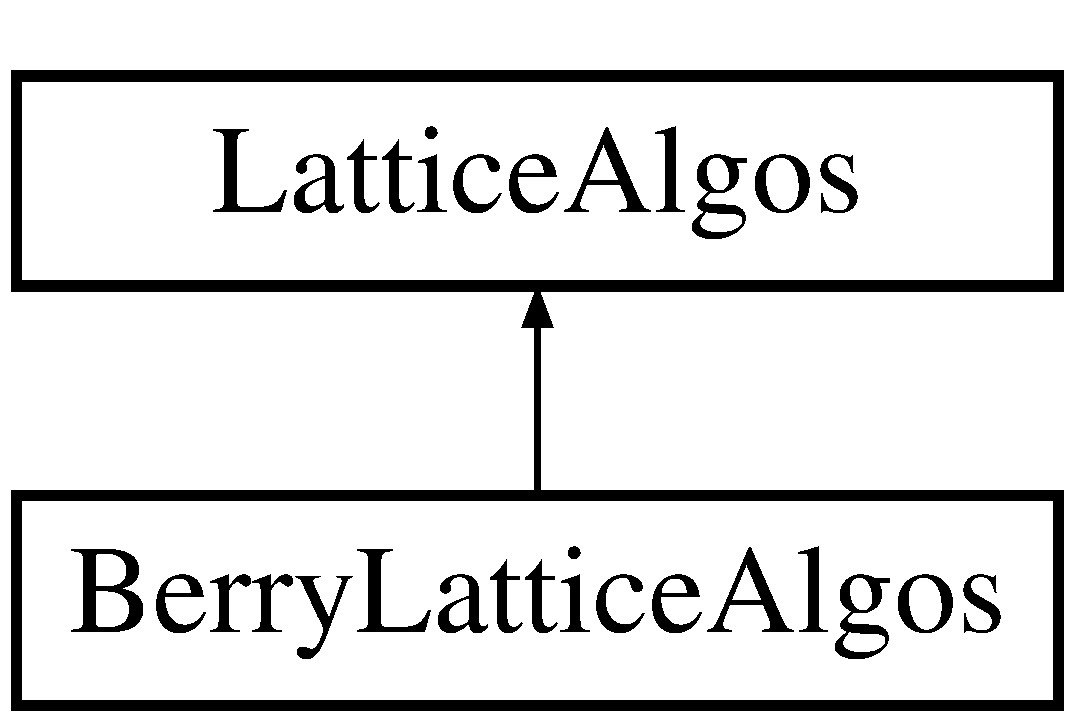
\includegraphics[height=2.000000cm]{class_lattice_algos}
\end{center}
\end{figure}
\subsection*{Public Member Functions}
\begin{DoxyCompactItemize}
\item 
\hyperlink{class_lattice_algos_ae3f96fdf1928948a830de0ec273534c1}{LatticeAlgos} ()
\begin{DoxyCompactList}\small\item\em Default constructor. \item\end{DoxyCompactList}\end{DoxyCompactItemize}
\subsection*{Public Attributes}
\begin{DoxyCompactItemize}
\item 
int \hyperlink{class_lattice_algos_a7061dd2e2590fa24e0dfb16f28509dce}{srchLvl}
\begin{DoxyCompactList}\small\item\em keeps track of the search level in an enumeration algorithm \item\end{DoxyCompactList}\item 
int \hyperlink{class_lattice_algos_a8a6e4d766e7f93a288e015e93b3183a0}{numConcepts}
\begin{DoxyCompactList}\small\item\em keeps track of the total number of concepts or clusters enumerated \item\end{DoxyCompactList}\item 
bool \hyperlink{class_lattice_algos_a7c599d38a3a66b926d7345153ca2e93c}{dispProgress}
\begin{DoxyCompactList}\small\item\em flag to indicate if progress of the algorithm should output to the user (stdout) \item\end{DoxyCompactList}\item 
vector$<$ \hyperlink{class_n_cluster}{NCluster} $\ast$ $>$ \hyperlink{class_lattice_algos_a006fbb44cdb89ab949bc9f47ed20a6d3}{CONCEPTS}
\begin{DoxyCompactList}\small\item\em data structure to hold the enumerated clusters in memory during algorithm exectuion \item\end{DoxyCompactList}\item 
vector$<$ \hyperlink{class_name_map}{NameMap} $\ast$ $>$ \hyperlink{class_lattice_algos_a242b1f9b2ec58cec08c4c5c074c0c1e7}{NAME\_\-MAPS}
\begin{DoxyCompactList}\small\item\em vector of name maps to be used to output clusters \item\end{DoxyCompactList}\item 
string \hyperlink{class_lattice_algos_aaf79cc2e8513fd28bf1e9329c3e678ab}{OUTFILE}
\begin{DoxyCompactList}\small\item\em if ENUM\_\-FILE or ENUM\_\-TOPK\_\-FILE is selected then this file is used to output the concepts \item\end{DoxyCompactList}\item 
ofstream \hyperlink{class_lattice_algos_a5e06ea8a8e76d5b6019481e778655a5c}{OUT1}
\begin{DoxyCompactList}\small\item\em ofstream used to output to OUTFILE.concepts \item\end{DoxyCompactList}\item 
ofstream \hyperlink{class_lattice_algos_ad6ee83e69ef859717cbc747edf4fc306}{OUT2}
\begin{DoxyCompactList}\small\item\em ofsteram used to output to OUTFILE.concept.names \item\end{DoxyCompactList}\item 
int \hyperlink{class_lattice_algos_a03adc61166377c993b4d1ef8f8ee12ee}{enumerationMode}
\begin{DoxyCompactList}\small\item\em Users will set this variable to indicate the enumeration mode. \item\end{DoxyCompactList}\item 
int \hyperlink{class_lattice_algos_aabdafd3fa45b3ed1d773b313e3a60e17}{qualityMode}
\begin{DoxyCompactList}\small\item\em user will set this variable to indicate the desired qualityMode \item\end{DoxyCompactList}\item 
double($\ast$ \hyperlink{class_lattice_algos_ae25f31284b5956278f390d0edc412ef8}{qualityFunction} )(\hyperlink{class_n_cluster}{NCluster} $\ast$, vector$<$ double $>$ \&)
\begin{DoxyCompactList}\small\item\em function pointer to a quality measure, interface functions will set this acrroding to qualityMode \item\end{DoxyCompactList}\item 
vector$<$ double $>$ \hyperlink{class_lattice_algos_a84a7c48411084ff5d792af41e57ce96a}{params}
\begin{DoxyCompactList}\small\item\em store the parameters for a quality function here, see the \hyperlink{_quality_measures_8h}{QualityMeasures.h} documentation for specification of these parameters \item\end{DoxyCompactList}\item 
int \hyperlink{class_lattice_algos_a7a9a7568a564e929c494c7c94ed5dda5}{ovlpMode}
\begin{DoxyCompactList}\small\item\em user will set this variable to inidicate the desired qualityMode \item\end{DoxyCompactList}\item 
double($\ast$ \hyperlink{class_lattice_algos_ad2bd9f8cb22cb27dfe527dd2bc38ec2d}{ovlpFunction} )(\hyperlink{class_n_cluster}{NCluster} $\ast$, \hyperlink{class_n_cluster}{NCluster} $\ast$)
\begin{DoxyCompactList}\small\item\em function pointer to an overlap function computer, interface function will set this according to ovlpMode \item\end{DoxyCompactList}\item 
double \hyperlink{class_lattice_algos_ae50e2eab1478e1bced92b0f1f1bcdc09}{ovlpThresh}
\begin{DoxyCompactList}\small\item\em a threshold value that indicates how much overlap two clusters may have before an algorithm keeps the higher quality cluster \item\end{DoxyCompactList}\item 
int \hyperlink{class_lattice_algos_a90e06533d513efc4635905624283eeae}{topKK}
\begin{DoxyCompactList}\small\item\em the number of clusters an algorithm should enumerate if user only wants the top k clusters \item\end{DoxyCompactList}\item 
int \hyperlink{class_lattice_algos_a5a4badfea96f02f89d8943ca7fecc2ab}{pruneMode}
\begin{DoxyCompactList}\small\item\em user will set this variable to indicate the the desired pruning mode \item\end{DoxyCompactList}\item 
vector$<$ int $>$ \hyperlink{class_lattice_algos_a244d9a63307846c2df232091a78a6759}{PRUNE\_\-SIZE\_\-VECTOR}
\begin{DoxyCompactList}\small\item\em if PRUNE\_\-SIZE mode is selected this vector should be initialized to the min support of each domain \item\end{DoxyCompactList}\end{DoxyCompactItemize}
\subsection*{Static Public Attributes}
\begin{DoxyCompactItemize}
\item 
static const int \hyperlink{class_lattice_algos_a80df6360d3246d74ae31e51e6c4bfa0e}{ENUM\_\-MEM} = 1
\begin{DoxyCompactList}\small\item\em Enumeration mode that specifies to algorithms to mine and store clusters in memory. \item\end{DoxyCompactList}\item 
static const int \hyperlink{class_lattice_algos_a824804a33640782553f2b399b28fde13}{ENUM\_\-FILE} = 2
\begin{DoxyCompactList}\small\item\em Enumeration mode that specifies to algorithms to mine and output clusters to a file, this file is specified by OUTFILE. \item\end{DoxyCompactList}\item 
static const int \hyperlink{class_lattice_algos_a04a0ea3a71c5b598242fa4ec3d4fce79}{ENUM\_\-TOPK\_\-FILE} = 3
\begin{DoxyCompactList}\small\item\em Enumeration mode that specifies to algorithms to mine only the top K clusters and output to a file, this file is specified by OUTFILE. \item\end{DoxyCompactList}\item 
static const int \hyperlink{class_lattice_algos_a1c6a4b5dce3ccade9e17ce4b2a6afbe7}{ENUM\_\-TOPK\_\-MEM} = 4
\begin{DoxyCompactList}\small\item\em Enumeration mode that specifies to algorithms to mine only the top K clusters and store in memory. \item\end{DoxyCompactList}\item 
static const int \hyperlink{class_lattice_algos_a0a79ddaab00906dea5756ac05a4861a5}{AREA} = 1
\begin{DoxyCompactList}\small\item\em quality mode that indicates to use the area of a concept as its quality measure \item\end{DoxyCompactList}\item 
static const int \hyperlink{class_lattice_algos_a3cf765cdc6bce759203597708324ee9e}{BETA} = 2
\begin{DoxyCompactList}\small\item\em quality mode that indicates to use the beta area of a concept as its quality measure (see \char`\"{}An effective algorithm for mining 3-\/clusters\char`\"{} by Alqadah et al.) \item\end{DoxyCompactList}\item 
static const int \hyperlink{class_lattice_algos_a24156b300d4b23d0d618f548091d0aeb}{AVG\_\-JACCARD} = 1
\begin{DoxyCompactList}\small\item\em overlap mode that indicates to use the average jaccard coefficient across all sets of an n-\/cluster to compute overlapping \item\end{DoxyCompactList}\item 
static const int \hyperlink{class_lattice_algos_a9a1d69347724b131f372706322776bbb}{PRUNE\_\-SIZE} = 1
\begin{DoxyCompactList}\small\item\em prune mode that indicates pruning will be based on size (support pruning) \item\end{DoxyCompactList}\end{DoxyCompactItemize}


\subsection{Detailed Description}


Definition at line 29 of file LatticeAlgos.h.



\subsection{Constructor \& Destructor Documentation}
\hypertarget{class_lattice_algos_ae3f96fdf1928948a830de0ec273534c1}{
\index{LatticeAlgos@{LatticeAlgos}!LatticeAlgos@{LatticeAlgos}}
\index{LatticeAlgos@{LatticeAlgos}!LatticeAlgos@{LatticeAlgos}}
\subsubsection[{LatticeAlgos}]{\setlength{\rightskip}{0pt plus 5cm}LatticeAlgos::LatticeAlgos (
\begin{DoxyParamCaption}
{}
\end{DoxyParamCaption}
)\hspace{0.3cm}{\ttfamily  \mbox{[}inline\mbox{]}}}}
\label{class_lattice_algos_ae3f96fdf1928948a830de0ec273534c1}


Default constructor. 



Definition at line 34 of file LatticeAlgos.h.



\subsection{Member Data Documentation}
\hypertarget{class_lattice_algos_a0a79ddaab00906dea5756ac05a4861a5}{
\index{LatticeAlgos@{LatticeAlgos}!AREA@{AREA}}
\index{AREA@{AREA}!LatticeAlgos@{LatticeAlgos}}
\subsubsection[{AREA}]{\setlength{\rightskip}{0pt plus 5cm}const int {\bf LatticeAlgos::AREA} = 1\hspace{0.3cm}{\ttfamily  \mbox{[}static\mbox{]}}}}
\label{class_lattice_algos_a0a79ddaab00906dea5756ac05a4861a5}


quality mode that indicates to use the area of a concept as its quality measure 



Definition at line 87 of file LatticeAlgos.h.

\hypertarget{class_lattice_algos_a24156b300d4b23d0d618f548091d0aeb}{
\index{LatticeAlgos@{LatticeAlgos}!AVG\_\-JACCARD@{AVG\_\-JACCARD}}
\index{AVG\_\-JACCARD@{AVG\_\-JACCARD}!LatticeAlgos@{LatticeAlgos}}
\subsubsection[{AVG\_\-JACCARD}]{\setlength{\rightskip}{0pt plus 5cm}const int {\bf LatticeAlgos::AVG\_\-JACCARD} = 1\hspace{0.3cm}{\ttfamily  \mbox{[}static\mbox{]}}}}
\label{class_lattice_algos_a24156b300d4b23d0d618f548091d0aeb}


overlap mode that indicates to use the average jaccard coefficient across all sets of an n-\/cluster to compute overlapping 



Definition at line 99 of file LatticeAlgos.h.

\hypertarget{class_lattice_algos_a3cf765cdc6bce759203597708324ee9e}{
\index{LatticeAlgos@{LatticeAlgos}!BETA@{BETA}}
\index{BETA@{BETA}!LatticeAlgos@{LatticeAlgos}}
\subsubsection[{BETA}]{\setlength{\rightskip}{0pt plus 5cm}const int {\bf LatticeAlgos::BETA} = 2\hspace{0.3cm}{\ttfamily  \mbox{[}static\mbox{]}}}}
\label{class_lattice_algos_a3cf765cdc6bce759203597708324ee9e}


quality mode that indicates to use the beta area of a concept as its quality measure (see \char`\"{}An effective algorithm for mining 3-\/clusters\char`\"{} by Alqadah et al.) 



Definition at line 89 of file LatticeAlgos.h.

\hypertarget{class_lattice_algos_a006fbb44cdb89ab949bc9f47ed20a6d3}{
\index{LatticeAlgos@{LatticeAlgos}!CONCEPTS@{CONCEPTS}}
\index{CONCEPTS@{CONCEPTS}!LatticeAlgos@{LatticeAlgos}}
\subsubsection[{CONCEPTS}]{\setlength{\rightskip}{0pt plus 5cm}vector$<${\bf NCluster}$\ast$$>$ {\bf LatticeAlgos::CONCEPTS}}}
\label{class_lattice_algos_a006fbb44cdb89ab949bc9f47ed20a6d3}


data structure to hold the enumerated clusters in memory during algorithm exectuion 



Definition at line 62 of file LatticeAlgos.h.

\hypertarget{class_lattice_algos_a7c599d38a3a66b926d7345153ca2e93c}{
\index{LatticeAlgos@{LatticeAlgos}!dispProgress@{dispProgress}}
\index{dispProgress@{dispProgress}!LatticeAlgos@{LatticeAlgos}}
\subsubsection[{dispProgress}]{\setlength{\rightskip}{0pt plus 5cm}bool {\bf LatticeAlgos::dispProgress}}}
\label{class_lattice_algos_a7c599d38a3a66b926d7345153ca2e93c}


flag to indicate if progress of the algorithm should output to the user (stdout) 



Definition at line 58 of file LatticeAlgos.h.

\hypertarget{class_lattice_algos_a824804a33640782553f2b399b28fde13}{
\index{LatticeAlgos@{LatticeAlgos}!ENUM\_\-FILE@{ENUM\_\-FILE}}
\index{ENUM\_\-FILE@{ENUM\_\-FILE}!LatticeAlgos@{LatticeAlgos}}
\subsubsection[{ENUM\_\-FILE}]{\setlength{\rightskip}{0pt plus 5cm}const int {\bf LatticeAlgos::ENUM\_\-FILE} = 2\hspace{0.3cm}{\ttfamily  \mbox{[}static\mbox{]}}}}
\label{class_lattice_algos_a824804a33640782553f2b399b28fde13}


Enumeration mode that specifies to algorithms to mine and output clusters to a file, this file is specified by OUTFILE. 



Definition at line 77 of file LatticeAlgos.h.

\hypertarget{class_lattice_algos_a80df6360d3246d74ae31e51e6c4bfa0e}{
\index{LatticeAlgos@{LatticeAlgos}!ENUM\_\-MEM@{ENUM\_\-MEM}}
\index{ENUM\_\-MEM@{ENUM\_\-MEM}!LatticeAlgos@{LatticeAlgos}}
\subsubsection[{ENUM\_\-MEM}]{\setlength{\rightskip}{0pt plus 5cm}const int {\bf LatticeAlgos::ENUM\_\-MEM} = 1\hspace{0.3cm}{\ttfamily  \mbox{[}static\mbox{]}}}}
\label{class_lattice_algos_a80df6360d3246d74ae31e51e6c4bfa0e}


Enumeration mode that specifies to algorithms to mine and store clusters in memory. 



Definition at line 75 of file LatticeAlgos.h.

\hypertarget{class_lattice_algos_a04a0ea3a71c5b598242fa4ec3d4fce79}{
\index{LatticeAlgos@{LatticeAlgos}!ENUM\_\-TOPK\_\-FILE@{ENUM\_\-TOPK\_\-FILE}}
\index{ENUM\_\-TOPK\_\-FILE@{ENUM\_\-TOPK\_\-FILE}!LatticeAlgos@{LatticeAlgos}}
\subsubsection[{ENUM\_\-TOPK\_\-FILE}]{\setlength{\rightskip}{0pt plus 5cm}const int {\bf LatticeAlgos::ENUM\_\-TOPK\_\-FILE} = 3\hspace{0.3cm}{\ttfamily  \mbox{[}static\mbox{]}}}}
\label{class_lattice_algos_a04a0ea3a71c5b598242fa4ec3d4fce79}


Enumeration mode that specifies to algorithms to mine only the top K clusters and output to a file, this file is specified by OUTFILE. 



Definition at line 79 of file LatticeAlgos.h.

\hypertarget{class_lattice_algos_a1c6a4b5dce3ccade9e17ce4b2a6afbe7}{
\index{LatticeAlgos@{LatticeAlgos}!ENUM\_\-TOPK\_\-MEM@{ENUM\_\-TOPK\_\-MEM}}
\index{ENUM\_\-TOPK\_\-MEM@{ENUM\_\-TOPK\_\-MEM}!LatticeAlgos@{LatticeAlgos}}
\subsubsection[{ENUM\_\-TOPK\_\-MEM}]{\setlength{\rightskip}{0pt plus 5cm}const int {\bf LatticeAlgos::ENUM\_\-TOPK\_\-MEM} = 4\hspace{0.3cm}{\ttfamily  \mbox{[}static\mbox{]}}}}
\label{class_lattice_algos_a1c6a4b5dce3ccade9e17ce4b2a6afbe7}


Enumeration mode that specifies to algorithms to mine only the top K clusters and store in memory. 



Definition at line 81 of file LatticeAlgos.h.

\hypertarget{class_lattice_algos_a03adc61166377c993b4d1ef8f8ee12ee}{
\index{LatticeAlgos@{LatticeAlgos}!enumerationMode@{enumerationMode}}
\index{enumerationMode@{enumerationMode}!LatticeAlgos@{LatticeAlgos}}
\subsubsection[{enumerationMode}]{\setlength{\rightskip}{0pt plus 5cm}int {\bf LatticeAlgos::enumerationMode}}}
\label{class_lattice_algos_a03adc61166377c993b4d1ef8f8ee12ee}


Users will set this variable to indicate the enumeration mode. 



Definition at line 83 of file LatticeAlgos.h.

\hypertarget{class_lattice_algos_a242b1f9b2ec58cec08c4c5c074c0c1e7}{
\index{LatticeAlgos@{LatticeAlgos}!NAME\_\-MAPS@{NAME\_\-MAPS}}
\index{NAME\_\-MAPS@{NAME\_\-MAPS}!LatticeAlgos@{LatticeAlgos}}
\subsubsection[{NAME\_\-MAPS}]{\setlength{\rightskip}{0pt plus 5cm}vector$<${\bf NameMap}$\ast$$>$ {\bf LatticeAlgos::NAME\_\-MAPS}}}
\label{class_lattice_algos_a242b1f9b2ec58cec08c4c5c074c0c1e7}


vector of name maps to be used to output clusters 



Definition at line 64 of file LatticeAlgos.h.

\hypertarget{class_lattice_algos_a8a6e4d766e7f93a288e015e93b3183a0}{
\index{LatticeAlgos@{LatticeAlgos}!numConcepts@{numConcepts}}
\index{numConcepts@{numConcepts}!LatticeAlgos@{LatticeAlgos}}
\subsubsection[{numConcepts}]{\setlength{\rightskip}{0pt plus 5cm}int {\bf LatticeAlgos::numConcepts}}}
\label{class_lattice_algos_a8a6e4d766e7f93a288e015e93b3183a0}


keeps track of the total number of concepts or clusters enumerated 



Definition at line 56 of file LatticeAlgos.h.

\hypertarget{class_lattice_algos_a5e06ea8a8e76d5b6019481e778655a5c}{
\index{LatticeAlgos@{LatticeAlgos}!OUT1@{OUT1}}
\index{OUT1@{OUT1}!LatticeAlgos@{LatticeAlgos}}
\subsubsection[{OUT1}]{\setlength{\rightskip}{0pt plus 5cm}ofstream {\bf LatticeAlgos::OUT1}}}
\label{class_lattice_algos_a5e06ea8a8e76d5b6019481e778655a5c}


ofstream used to output to OUTFILE.concepts 



Definition at line 68 of file LatticeAlgos.h.

\hypertarget{class_lattice_algos_ad6ee83e69ef859717cbc747edf4fc306}{
\index{LatticeAlgos@{LatticeAlgos}!OUT2@{OUT2}}
\index{OUT2@{OUT2}!LatticeAlgos@{LatticeAlgos}}
\subsubsection[{OUT2}]{\setlength{\rightskip}{0pt plus 5cm}ofstream {\bf LatticeAlgos::OUT2}}}
\label{class_lattice_algos_ad6ee83e69ef859717cbc747edf4fc306}


ofsteram used to output to OUTFILE.concept.names 



Definition at line 70 of file LatticeAlgos.h.

\hypertarget{class_lattice_algos_aaf79cc2e8513fd28bf1e9329c3e678ab}{
\index{LatticeAlgos@{LatticeAlgos}!OUTFILE@{OUTFILE}}
\index{OUTFILE@{OUTFILE}!LatticeAlgos@{LatticeAlgos}}
\subsubsection[{OUTFILE}]{\setlength{\rightskip}{0pt plus 5cm}string {\bf LatticeAlgos::OUTFILE}}}
\label{class_lattice_algos_aaf79cc2e8513fd28bf1e9329c3e678ab}


if ENUM\_\-FILE or ENUM\_\-TOPK\_\-FILE is selected then this file is used to output the concepts 



Definition at line 66 of file LatticeAlgos.h.

\hypertarget{class_lattice_algos_ad2bd9f8cb22cb27dfe527dd2bc38ec2d}{
\index{LatticeAlgos@{LatticeAlgos}!ovlpFunction@{ovlpFunction}}
\index{ovlpFunction@{ovlpFunction}!LatticeAlgos@{LatticeAlgos}}
\subsubsection[{ovlpFunction}]{\setlength{\rightskip}{0pt plus 5cm}double($\ast$ {\bf LatticeAlgos::ovlpFunction})({\bf NCluster} $\ast$, {\bf NCluster} $\ast$)}}
\label{class_lattice_algos_ad2bd9f8cb22cb27dfe527dd2bc38ec2d}


function pointer to an overlap function computer, interface function will set this according to ovlpMode 



Definition at line 103 of file LatticeAlgos.h.

\hypertarget{class_lattice_algos_a7a9a7568a564e929c494c7c94ed5dda5}{
\index{LatticeAlgos@{LatticeAlgos}!ovlpMode@{ovlpMode}}
\index{ovlpMode@{ovlpMode}!LatticeAlgos@{LatticeAlgos}}
\subsubsection[{ovlpMode}]{\setlength{\rightskip}{0pt plus 5cm}int {\bf LatticeAlgos::ovlpMode}}}
\label{class_lattice_algos_a7a9a7568a564e929c494c7c94ed5dda5}


user will set this variable to inidicate the desired qualityMode 



Definition at line 101 of file LatticeAlgos.h.

\hypertarget{class_lattice_algos_ae50e2eab1478e1bced92b0f1f1bcdc09}{
\index{LatticeAlgos@{LatticeAlgos}!ovlpThresh@{ovlpThresh}}
\index{ovlpThresh@{ovlpThresh}!LatticeAlgos@{LatticeAlgos}}
\subsubsection[{ovlpThresh}]{\setlength{\rightskip}{0pt plus 5cm}double {\bf LatticeAlgos::ovlpThresh}}}
\label{class_lattice_algos_ae50e2eab1478e1bced92b0f1f1bcdc09}


a threshold value that indicates how much overlap two clusters may have before an algorithm keeps the higher quality cluster 



Definition at line 105 of file LatticeAlgos.h.

\hypertarget{class_lattice_algos_a84a7c48411084ff5d792af41e57ce96a}{
\index{LatticeAlgos@{LatticeAlgos}!params@{params}}
\index{params@{params}!LatticeAlgos@{LatticeAlgos}}
\subsubsection[{params}]{\setlength{\rightskip}{0pt plus 5cm}vector$<$double$>$ {\bf LatticeAlgos::params}}}
\label{class_lattice_algos_a84a7c48411084ff5d792af41e57ce96a}


store the parameters for a quality function here, see the \hyperlink{_quality_measures_8h}{QualityMeasures.h} documentation for specification of these parameters 



Definition at line 95 of file LatticeAlgos.h.

\hypertarget{class_lattice_algos_a9a1d69347724b131f372706322776bbb}{
\index{LatticeAlgos@{LatticeAlgos}!PRUNE\_\-SIZE@{PRUNE\_\-SIZE}}
\index{PRUNE\_\-SIZE@{PRUNE\_\-SIZE}!LatticeAlgos@{LatticeAlgos}}
\subsubsection[{PRUNE\_\-SIZE}]{\setlength{\rightskip}{0pt plus 5cm}const int {\bf LatticeAlgos::PRUNE\_\-SIZE} = 1\hspace{0.3cm}{\ttfamily  \mbox{[}static\mbox{]}}}}
\label{class_lattice_algos_a9a1d69347724b131f372706322776bbb}


prune mode that indicates pruning will be based on size (support pruning) 



Definition at line 113 of file LatticeAlgos.h.

\hypertarget{class_lattice_algos_a244d9a63307846c2df232091a78a6759}{
\index{LatticeAlgos@{LatticeAlgos}!PRUNE\_\-SIZE\_\-VECTOR@{PRUNE\_\-SIZE\_\-VECTOR}}
\index{PRUNE\_\-SIZE\_\-VECTOR@{PRUNE\_\-SIZE\_\-VECTOR}!LatticeAlgos@{LatticeAlgos}}
\subsubsection[{PRUNE\_\-SIZE\_\-VECTOR}]{\setlength{\rightskip}{0pt plus 5cm}vector$<$int$>$ {\bf LatticeAlgos::PRUNE\_\-SIZE\_\-VECTOR}}}
\label{class_lattice_algos_a244d9a63307846c2df232091a78a6759}


if PRUNE\_\-SIZE mode is selected this vector should be initialized to the min support of each domain 

PRUNE\_\-SIZE\_\-VECTOR\mbox{[}domainId-\/1\mbox{]} should contain the minumum number of objects a domain with domainId should contian in order to be considered for enumeration. Users must set the values for this vector 

Definition at line 122 of file LatticeAlgos.h.

\hypertarget{class_lattice_algos_a5a4badfea96f02f89d8943ca7fecc2ab}{
\index{LatticeAlgos@{LatticeAlgos}!pruneMode@{pruneMode}}
\index{pruneMode@{pruneMode}!LatticeAlgos@{LatticeAlgos}}
\subsubsection[{pruneMode}]{\setlength{\rightskip}{0pt plus 5cm}int {\bf LatticeAlgos::pruneMode}}}
\label{class_lattice_algos_a5a4badfea96f02f89d8943ca7fecc2ab}


user will set this variable to indicate the the desired pruning mode 



Definition at line 115 of file LatticeAlgos.h.

\hypertarget{class_lattice_algos_ae25f31284b5956278f390d0edc412ef8}{
\index{LatticeAlgos@{LatticeAlgos}!qualityFunction@{qualityFunction}}
\index{qualityFunction@{qualityFunction}!LatticeAlgos@{LatticeAlgos}}
\subsubsection[{qualityFunction}]{\setlength{\rightskip}{0pt plus 5cm}double($\ast$ {\bf LatticeAlgos::qualityFunction})({\bf NCluster} $\ast$, vector$<$ double $>$ \&)}}
\label{class_lattice_algos_ae25f31284b5956278f390d0edc412ef8}


function pointer to a quality measure, interface functions will set this acrroding to qualityMode 



Definition at line 93 of file LatticeAlgos.h.

\hypertarget{class_lattice_algos_aabdafd3fa45b3ed1d773b313e3a60e17}{
\index{LatticeAlgos@{LatticeAlgos}!qualityMode@{qualityMode}}
\index{qualityMode@{qualityMode}!LatticeAlgos@{LatticeAlgos}}
\subsubsection[{qualityMode}]{\setlength{\rightskip}{0pt plus 5cm}int {\bf LatticeAlgos::qualityMode}}}
\label{class_lattice_algos_aabdafd3fa45b3ed1d773b313e3a60e17}


user will set this variable to indicate the desired qualityMode 



Definition at line 91 of file LatticeAlgos.h.

\hypertarget{class_lattice_algos_a7061dd2e2590fa24e0dfb16f28509dce}{
\index{LatticeAlgos@{LatticeAlgos}!srchLvl@{srchLvl}}
\index{srchLvl@{srchLvl}!LatticeAlgos@{LatticeAlgos}}
\subsubsection[{srchLvl}]{\setlength{\rightskip}{0pt plus 5cm}int {\bf LatticeAlgos::srchLvl}}}
\label{class_lattice_algos_a7061dd2e2590fa24e0dfb16f28509dce}


keeps track of the search level in an enumeration algorithm 



Definition at line 54 of file LatticeAlgos.h.

\hypertarget{class_lattice_algos_a90e06533d513efc4635905624283eeae}{
\index{LatticeAlgos@{LatticeAlgos}!topKK@{topKK}}
\index{topKK@{topKK}!LatticeAlgos@{LatticeAlgos}}
\subsubsection[{topKK}]{\setlength{\rightskip}{0pt plus 5cm}int {\bf LatticeAlgos::topKK}}}
\label{class_lattice_algos_a90e06533d513efc4635905624283eeae}


the number of clusters an algorithm should enumerate if user only wants the top k clusters 



Definition at line 109 of file LatticeAlgos.h.



The documentation for this class was generated from the following file:\begin{DoxyCompactItemize}
\item 
/Users/alqadaf/Research/Code/core/headers/\hyperlink{_lattice_algos_8h}{LatticeAlgos.h}\end{DoxyCompactItemize}

\hypertarget{class_name_map}{
\section{NameMap Class Reference}
\label{class_name_map}\index{NameMap@{NameMap}}
}
\subsection*{Public Member Functions}
\begin{DoxyCompactItemize}
\item 
\hypertarget{class_name_map_a8560d4570112d839b90be032f2af34e7}{
\hyperlink{class_name_map_a8560d4570112d839b90be032f2af34e7}{NameMap} ()}
\label{class_name_map_a8560d4570112d839b90be032f2af34e7}

\begin{DoxyCompactList}\small\item\em Default constructor. No actual map is constructed, since no file is read. \item\end{DoxyCompactList}\item 
\hypertarget{class_name_map_a65b751a2cf738a2d391aca986d5f5281}{
\hyperlink{class_name_map_a65b751a2cf738a2d391aca986d5f5281}{NameMap} (string \&file)}
\label{class_name_map_a65b751a2cf738a2d391aca986d5f5281}

\begin{DoxyCompactList}\small\item\em Alternate constructor that passes in the file name and constructs the actual name map. \item\end{DoxyCompactList}\item 
\hypertarget{class_name_map_a4874c7a4e95a4dd589e834e12faa1999}{
\hyperlink{class_name_map_a4874c7a4e95a4dd589e834e12faa1999}{NameMap} (string, unsigned int n)}
\label{class_name_map_a4874c7a4e95a4dd589e834e12faa1999}

\begin{DoxyCompactList}\small\item\em Alternate constructor that passes in the file name and constructs the actual name map but only upto the nth entry. \item\end{DoxyCompactList}\item 
\hypertarget{class_name_map_a9b58a913f6abdda24ead4f56c36a75d4}{
string \hyperlink{class_name_map_a9b58a913f6abdda24ead4f56c36a75d4}{GetFileName} ()}
\label{class_name_map_a9b58a913f6abdda24ead4f56c36a75d4}

\begin{DoxyCompactList}\small\item\em Returns the file name from which the name map was constructed. \item\end{DoxyCompactList}\item 
\hypertarget{class_name_map_a0ceabf530c3093d6fa163932c928d7bf}{
string \hyperlink{class_name_map_a0ceabf530c3093d6fa163932c928d7bf}{GetName} (unsigned int i)}
\label{class_name_map_a0ceabf530c3093d6fa163932c928d7bf}

\begin{DoxyCompactList}\small\item\em returns the string mapped to i \item\end{DoxyCompactList}\item 
\hypertarget{class_name_map_ab1922430c9e4d12e67b5f27edf9afd15}{
int \hyperlink{class_name_map_ab1922430c9e4d12e67b5f27edf9afd15}{GetNumEntries} ()}
\label{class_name_map_ab1922430c9e4d12e67b5f27edf9afd15}

\begin{DoxyCompactList}\small\item\em Returns the number of entries in the map. \item\end{DoxyCompactList}\item 
\hypertarget{class_name_map_a61afb305b470bab4e3c9e14279d6f1c5}{
void \hyperlink{class_name_map_a61afb305b470bab4e3c9e14279d6f1c5}{SetId} (int)}
\label{class_name_map_a61afb305b470bab4e3c9e14279d6f1c5}

\begin{DoxyCompactList}\small\item\em Set the id attribute of the name map. \item\end{DoxyCompactList}\item 
\hypertarget{class_name_map_a5ec2b743e894000de9dcc0c7cf198775}{
int \hyperlink{class_name_map_a5ec2b743e894000de9dcc0c7cf198775}{GetId} ()}
\label{class_name_map_a5ec2b743e894000de9dcc0c7cf198775}

\begin{DoxyCompactList}\small\item\em Returns the id attribue of the name map. \item\end{DoxyCompactList}\end{DoxyCompactItemize}
\subsection*{Private Attributes}
\begin{DoxyCompactItemize}
\item 
\hypertarget{class_name_map_a1acb823b1c1fb7b8d43f7e0e1406dca8}{
vector$<$ string $>$ \hyperlink{class_name_map_a1acb823b1c1fb7b8d43f7e0e1406dca8}{mapping}}
\label{class_name_map_a1acb823b1c1fb7b8d43f7e0e1406dca8}

\begin{DoxyCompactList}\small\item\em the actual map, maps the index in the vector to the string \item\end{DoxyCompactList}\item 
\hypertarget{class_name_map_a647caae861e8a9e8472a033da6c0ad20}{
int \hyperlink{class_name_map_a647caae861e8a9e8472a033da6c0ad20}{numEntries}}
\label{class_name_map_a647caae861e8a9e8472a033da6c0ad20}

\begin{DoxyCompactList}\small\item\em number of entries \item\end{DoxyCompactList}\item 
\hypertarget{class_name_map_acf6827aa9176aa0820a2c7c0ec0cf3a4}{
string \hyperlink{class_name_map_acf6827aa9176aa0820a2c7c0ec0cf3a4}{fileName}}
\label{class_name_map_acf6827aa9176aa0820a2c7c0ec0cf3a4}

\begin{DoxyCompactList}\small\item\em name of the file from which the map was constructed \item\end{DoxyCompactList}\item 
\hypertarget{class_name_map_ab836a5099928fbf10c864504fd658fa8}{
int {\bfseries id}}
\label{class_name_map_ab836a5099928fbf10c864504fd658fa8}

\end{DoxyCompactItemize}


\subsection{Detailed Description}


Definition at line 22 of file NameMap.h.



The documentation for this class was generated from the following files:\begin{DoxyCompactItemize}
\item 
headers/NameMap.h\item 
source/NameMap.cpp\end{DoxyCompactItemize}

\hypertarget{class_n_cluster}{
\section{NCluster Class Reference}
\label{class_n_cluster}\index{NCluster@{NCluster}}
}
\subsection*{Public Member Functions}
\begin{DoxyCompactItemize}
\item 
\hypertarget{class_n_cluster_af90ad520f3efec3f3c0b93ba9f46debc}{
\hyperlink{class_n_cluster_af90ad520f3efec3f3c0b93ba9f46debc}{NCluster} ()}
\label{class_n_cluster_af90ad520f3efec3f3c0b93ba9f46debc}

\begin{DoxyCompactList}\small\item\em Default constructor. \item\end{DoxyCompactList}\item 
\hyperlink{class_n_cluster_ac6460cead5fb2cf1a46354ab26f36e0a}{NCluster} (unsigned int \hyperlink{class_n_cluster_a926e474ba279516160b52ab36d208a69}{n})
\begin{DoxyCompactList}\small\item\em Alternate constructor. \item\end{DoxyCompactList}\item 
\hyperlink{class_n_cluster_ad64a3005375dd6aad2848f227ce92ef6}{NCluster} (unsigned int \hyperlink{class_n_cluster_a926e474ba279516160b52ab36d208a69}{n}, bool allocate)
\begin{DoxyCompactList}\small\item\em Alternate constructor. \item\end{DoxyCompactList}\item 
\hyperlink{class_n_cluster_a5ef4833105e769e289f7e9dbf570dcef}{NCluster} (unsigned int \hyperlink{class_n_cluster_a926e474ba279516160b52ab36d208a69}{n}, vector$<$ \hyperlink{class_i_o_set}{IOSet} $\ast$ $>$ \&aa)
\begin{DoxyCompactList}\small\item\em Alternate constructor. \item\end{DoxyCompactList}\item 
\hypertarget{class_n_cluster_a7f86cfa4150010e117f7520f34bbc6a4}{
\hyperlink{class_n_cluster_a7f86cfa4150010e117f7520f34bbc6a4}{NCluster} (\hyperlink{class_n_cluster}{NCluster} \&)}
\label{class_n_cluster_a7f86cfa4150010e117f7520f34bbc6a4}

\begin{DoxyCompactList}\small\item\em Copy constructor. \item\end{DoxyCompactList}\item 
\hypertarget{class_n_cluster_aae72a31bc6c2f05934a6d2248d966be5}{
\hyperlink{class_n_cluster_aae72a31bc6c2f05934a6d2248d966be5}{$\sim$NCluster} ()}
\label{class_n_cluster_aae72a31bc6c2f05934a6d2248d966be5}

\begin{DoxyCompactList}\small\item\em Destructor. \item\end{DoxyCompactList}\item 
\hypertarget{class_n_cluster_a84dd370bb3e73f192187156cd7dba57b}{
void \hyperlink{class_n_cluster_a84dd370bb3e73f192187156cd7dba57b}{DeepCopy} (\hyperlink{class_n_cluster}{NCluster} \&)}
\label{class_n_cluster_a84dd370bb3e73f192187156cd7dba57b}

\begin{DoxyCompactList}\small\item\em Makes a deep copy of the n-\/cluster. \item\end{DoxyCompactList}\item 
\hypertarget{class_n_cluster_a695c426f13c2fb78015c2f6d8714dc38}{
void \hyperlink{class_n_cluster_a695c426f13c2fb78015c2f6d8714dc38}{Output} ()}
\label{class_n_cluster_a695c426f13c2fb78015c2f6d8714dc38}

\begin{DoxyCompactList}\small\item\em Prints each IOset on a seperate line preceded by the Id of each \hyperlink{class_i_o_set}{IOSet} to stdout. \item\end{DoxyCompactList}\item 
\hypertarget{class_n_cluster_afb92f84876326645c2d3e46c011c6fdf}{
void \hyperlink{class_n_cluster_afb92f84876326645c2d3e46c011c6fdf}{Output} (ofstream \&)}
\label{class_n_cluster_afb92f84876326645c2d3e46c011c6fdf}

\begin{DoxyCompactList}\small\item\em Prints each IOset on a seperate line preceded by the Id of each \hyperlink{class_i_o_set}{IOSet} to ofstream. \item\end{DoxyCompactList}\item 
void \hyperlink{class_n_cluster_a5f75034c596cda89b823bb842f54019e}{Output} (ofstream \&, vector$<$ \hyperlink{class_name_map}{NameMap} $\ast$ $>$ \&nm)
\begin{DoxyCompactList}\small\item\em Prints each IOset on a seperate line preceded by the Id of each \hyperlink{class_i_o_set}{IOSet} to ofstream. \item\end{DoxyCompactList}\item 
void \hyperlink{class_n_cluster_a762a3beaf5aa389d8afccabe227d30e3}{Output} (vector$<$ \hyperlink{class_name_map}{NameMap} $\ast$ $>$ \&nm)
\begin{DoxyCompactList}\small\item\em Prints each IOset on a seperate line preceded by the Id of each \hyperlink{class_i_o_set}{IOSet} to std stream. \item\end{DoxyCompactList}\item 
\hypertarget{class_n_cluster_a5e91f8c38a0122031c3f921b94e3a688}{
int \hyperlink{class_n_cluster_a5e91f8c38a0122031c3f921b94e3a688}{GetN} ()}
\label{class_n_cluster_a5e91f8c38a0122031c3f921b94e3a688}

\begin{DoxyCompactList}\small\item\em Resurns n, the number of sets in the n-\/cluster. \item\end{DoxyCompactList}\item 
\hypertarget{class_n_cluster_a7d197e1cf217fe1ce95b0ba0b4ee40bc}{
\hyperlink{class_i_o_set}{IOSet} $\ast$ \hyperlink{class_n_cluster_a7d197e1cf217fe1ce95b0ba0b4ee40bc}{GetSet} (int)}
\label{class_n_cluster_a7d197e1cf217fe1ce95b0ba0b4ee40bc}

\begin{DoxyCompactList}\small\item\em Returns a pointer to the ith set. \item\end{DoxyCompactList}\item 
\hypertarget{class_n_cluster_a5d4ddbb124fc5d9c9cc706312ec80476}{
\hyperlink{class_i_o_set}{IOSet} $\ast$ \hyperlink{class_n_cluster_a5d4ddbb124fc5d9c9cc706312ec80476}{GetSetById} (int \hyperlink{class_n_cluster_a9360cadd4e338b91de61f86997acc890}{id})}
\label{class_n_cluster_a5d4ddbb124fc5d9c9cc706312ec80476}

\begin{DoxyCompactList}\small\item\em Returns a pointer to the set with id, if it exists, assertion is checked. \item\end{DoxyCompactList}\item 
\hypertarget{class_n_cluster_af4eeecc0717c16ffaa931a0100739f31}{
void \hyperlink{class_n_cluster_af4eeecc0717c16ffaa931a0100739f31}{AddSet} (\hyperlink{class_i_o_set}{IOSet} $\ast$a)}
\label{class_n_cluster_af4eeecc0717c16ffaa931a0100739f31}

\begin{DoxyCompactList}\small\item\em Adds the set a to the end of the n-\/cluster. \item\end{DoxyCompactList}\item 
\hypertarget{class_n_cluster_a7d5ab8fb3293b472b57cb9e964f5b90e}{
void \hyperlink{class_n_cluster_a7d5ab8fb3293b472b57cb9e964f5b90e}{AssignSet} (int i, \hyperlink{class_i_o_set}{IOSet} $\ast$a)}
\label{class_n_cluster_a7d5ab8fb3293b472b57cb9e964f5b90e}

\begin{DoxyCompactList}\small\item\em Assigns a to the ith, deleting the previously defined ith set in the process. \item\end{DoxyCompactList}\item 
\hypertarget{class_n_cluster_a0b117e61aee299f09f385f0b890bf0e1}{
void \hyperlink{class_n_cluster_a0b117e61aee299f09f385f0b890bf0e1}{AssignSetById} (int \hyperlink{class_n_cluster_a9360cadd4e338b91de61f86997acc890}{id}, \hyperlink{class_i_o_set}{IOSet} $\ast$a)}
\label{class_n_cluster_a0b117e61aee299f09f385f0b890bf0e1}

\begin{DoxyCompactList}\small\item\em Assigns a to the set with id, if it exists, previoulsy defined set with id is destroyed in the process. \item\end{DoxyCompactList}\item 
\hypertarget{class_n_cluster_aad3afb3c6ca495bd69fe0593455ca785}{
double \hyperlink{class_n_cluster_aad3afb3c6ca495bd69fe0593455ca785}{GetQuality} ()}
\label{class_n_cluster_aad3afb3c6ca495bd69fe0593455ca785}

\begin{DoxyCompactList}\small\item\em Returns the quality attribute. \item\end{DoxyCompactList}\item 
\hypertarget{class_n_cluster_abf7185a77e66f15d4ff3b400d51d1064}{
void \hyperlink{class_n_cluster_abf7185a77e66f15d4ff3b400d51d1064}{SetQuality} (double)}
\label{class_n_cluster_abf7185a77e66f15d4ff3b400d51d1064}

\begin{DoxyCompactList}\small\item\em Set the quality attribute. \item\end{DoxyCompactList}\item 
\hypertarget{class_n_cluster_a185204e735f03d9670855e0767592149}{
int \hyperlink{class_n_cluster_a185204e735f03d9670855e0767592149}{GetId} ()}
\label{class_n_cluster_a185204e735f03d9670855e0767592149}

\begin{DoxyCompactList}\small\item\em Returns the id attribute. \item\end{DoxyCompactList}\item 
\hypertarget{class_n_cluster_a62df66a6ed98f118dcdfebe3dc1fced5}{
void \hyperlink{class_n_cluster_a62df66a6ed98f118dcdfebe3dc1fced5}{SetId} (int)}
\label{class_n_cluster_a62df66a6ed98f118dcdfebe3dc1fced5}

\begin{DoxyCompactList}\small\item\em Set the id attribute. \item\end{DoxyCompactList}\item 
\hypertarget{class_n_cluster_a81e298f10335141a1257d29dc4c2e705}{
bool \hyperlink{class_n_cluster_a81e298f10335141a1257d29dc4c2e705}{GetMarked} ()}
\label{class_n_cluster_a81e298f10335141a1257d29dc4c2e705}

\begin{DoxyCompactList}\small\item\em Return the marked attribute. \item\end{DoxyCompactList}\item 
\hypertarget{class_n_cluster_abb8e5da62c63785a3ac9f4ab3aad207e}{
void \hyperlink{class_n_cluster_abb8e5da62c63785a3ac9f4ab3aad207e}{SetMarked} (bool m)}
\label{class_n_cluster_abb8e5da62c63785a3ac9f4ab3aad207e}

\begin{DoxyCompactList}\small\item\em Set the marked attribute. \item\end{DoxyCompactList}\item 
\hypertarget{class_n_cluster_acf1d8f02e7b8ec537225e896ae26534c}{
bool \hyperlink{class_n_cluster_acf1d8f02e7b8ec537225e896ae26534c}{ContainsIOSetId} (int \hyperlink{class_n_cluster_a9360cadd4e338b91de61f86997acc890}{id})}
\label{class_n_cluster_acf1d8f02e7b8ec537225e896ae26534c}

\begin{DoxyCompactList}\small\item\em Returns true if an \hyperlink{class_i_o_set}{IOSet} with id=id exists in self, false otherwsie. \item\end{DoxyCompactList}\item 
\hypertarget{class_n_cluster_a35ad64188494aec6b0b5a255217ba11b}{
int \hyperlink{class_n_cluster_a35ad64188494aec6b0b5a255217ba11b}{GetMaxElement} ()}
\label{class_n_cluster_a35ad64188494aec6b0b5a255217ba11b}

\begin{DoxyCompactList}\small\item\em Returns the value of the largest element in all sets of self. \item\end{DoxyCompactList}\item 
\hypertarget{class_n_cluster_a3cea2ce61b20d00b751041984660eba5}{
void \hyperlink{class_n_cluster_a3cea2ce61b20d00b751041984660eba5}{RemoveSet} (int i)}
\label{class_n_cluster_a3cea2ce61b20d00b751041984660eba5}

\begin{DoxyCompactList}\small\item\em Remove the \hyperlink{class_i_o_set}{IOSet} at index i. \item\end{DoxyCompactList}\item 
\hypertarget{class_n_cluster_a977c14300769c0146dbb5b0fa8773a08}{
void \hyperlink{class_n_cluster_a977c14300769c0146dbb5b0fa8773a08}{SortSets} ()}
\label{class_n_cluster_a977c14300769c0146dbb5b0fa8773a08}

\begin{DoxyCompactList}\small\item\em Sort the sets by the quality variables of each \hyperlink{class_i_o_set}{IOSet}. \item\end{DoxyCompactList}\end{DoxyCompactItemize}
\subsection*{Protected Attributes}
\begin{DoxyCompactItemize}
\item 
\hypertarget{class_n_cluster_a926e474ba279516160b52ab36d208a69}{
unsigned int \hyperlink{class_n_cluster_a926e474ba279516160b52ab36d208a69}{n}}
\label{class_n_cluster_a926e474ba279516160b52ab36d208a69}

\begin{DoxyCompactList}\small\item\em degree of the cluster \item\end{DoxyCompactList}\item 
\hypertarget{class_n_cluster_a2333af10251a6a884395aab57b9fa400}{
vector$<$ \hyperlink{class_i_o_set}{IOSet} $\ast$ $>$ \hyperlink{class_n_cluster_a2333af10251a6a884395aab57b9fa400}{sets}}
\label{class_n_cluster_a2333af10251a6a884395aab57b9fa400}

\begin{DoxyCompactList}\small\item\em the actual data or sets \item\end{DoxyCompactList}\item 
\hypertarget{class_n_cluster_a9e0aa868b02c27e6c282f9633a135aa9}{
double \hyperlink{class_n_cluster_a9e0aa868b02c27e6c282f9633a135aa9}{quality}}
\label{class_n_cluster_a9e0aa868b02c27e6c282f9633a135aa9}

\begin{DoxyCompactList}\small\item\em quality of the n-\/cluster \item\end{DoxyCompactList}\item 
\hypertarget{class_n_cluster_a9360cadd4e338b91de61f86997acc890}{
int \hyperlink{class_n_cluster_a9360cadd4e338b91de61f86997acc890}{id}}
\label{class_n_cluster_a9360cadd4e338b91de61f86997acc890}

\begin{DoxyCompactList}\small\item\em id of the n-\/cluster \item\end{DoxyCompactList}\item 
\hypertarget{class_n_cluster_a89a39f622490f47ed6283b17fe1d0f44}{
bool \hyperlink{class_n_cluster_a89a39f622490f47ed6283b17fe1d0f44}{marked}}
\label{class_n_cluster_a89a39f622490f47ed6283b17fe1d0f44}

\begin{DoxyCompactList}\small\item\em has this n-\/cluster been marked or flagged for whatever reason?? \item\end{DoxyCompactList}\end{DoxyCompactItemize}


\subsection{Detailed Description}


Definition at line 13 of file NCluster.h.



\subsection{Constructor \& Destructor Documentation}
\hypertarget{class_n_cluster_ac6460cead5fb2cf1a46354ab26f36e0a}{
\index{NCluster@{NCluster}!NCluster@{NCluster}}
\index{NCluster@{NCluster}!NCluster@{NCluster}}
\subsubsection[{NCluster}]{\setlength{\rightskip}{0pt plus 5cm}NCluster::NCluster (unsigned int {\em n})}}
\label{class_n_cluster_ac6460cead5fb2cf1a46354ab26f36e0a}


Alternate constructor. 

Allocates n sets and sets size to n 
\begin{DoxyParams}{Parameters}
\item[{\em n}]number of sets to allocate \end{DoxyParams}


Definition at line 9 of file NCluster.cpp.

\hypertarget{class_n_cluster_ad64a3005375dd6aad2848f227ce92ef6}{
\index{NCluster@{NCluster}!NCluster@{NCluster}}
\index{NCluster@{NCluster}!NCluster@{NCluster}}
\subsubsection[{NCluster}]{\setlength{\rightskip}{0pt plus 5cm}NCluster::NCluster (unsigned int {\em n}, \/  bool {\em allocate})}}
\label{class_n_cluster_ad64a3005375dd6aad2848f227ce92ef6}


Alternate constructor. 

Makes the n-\/cluster of size n, but does not allocate the memory 
\begin{DoxyParams}{Parameters}
\item[{\em n}]size of the n-\/cluster \item[{\em allocate}]this value does not matter, if its true or false, its just to inidcate that no memory should be allocated \end{DoxyParams}


Definition at line 27 of file NCluster.cpp.

\hypertarget{class_n_cluster_a5ef4833105e769e289f7e9dbf570dcef}{
\index{NCluster@{NCluster}!NCluster@{NCluster}}
\index{NCluster@{NCluster}!NCluster@{NCluster}}
\subsubsection[{NCluster}]{\setlength{\rightskip}{0pt plus 5cm}NCluster::NCluster (unsigned int {\em n}, \/  vector$<$ {\bf IOSet} $\ast$ $>$ \& {\em aa})}}
\label{class_n_cluster_a5ef4833105e769e289f7e9dbf570dcef}


Alternate constructor. 

Constructor n-\/cluster of size n and assigin a deep copy of the IOsets from the vector aa to the n-\/cluster  n size of the n-\/cluster  aa a vector of IOSets that will be used to initialize the sets of self by making a deep copy 

Definition at line 17 of file NCluster.cpp.



\subsection{Member Function Documentation}
\hypertarget{class_n_cluster_a762a3beaf5aa389d8afccabe227d30e3}{
\index{NCluster@{NCluster}!Output@{Output}}
\index{Output@{Output}!NCluster@{NCluster}}
\subsubsection[{Output}]{\setlength{\rightskip}{0pt plus 5cm}void NCluster::Output (vector$<$ {\bf NameMap} $\ast$ $>$ \& {\em nm})}}
\label{class_n_cluster_a762a3beaf5aa389d8afccabe227d30e3}


Prints each IOset on a seperate line preceded by the Id of each \hyperlink{class_i_o_set}{IOSet} to std stream. 

Attempts to match the id of one of the name maps to the id of the sets of self. If the ids match, then then \hyperlink{class_i_o_set}{IOSet} is output using the name map, otherwise normal printing is performed. 

Definition at line 94 of file NCluster.cpp.

\hypertarget{class_n_cluster_a5f75034c596cda89b823bb842f54019e}{
\index{NCluster@{NCluster}!Output@{Output}}
\index{Output@{Output}!NCluster@{NCluster}}
\subsubsection[{Output}]{\setlength{\rightskip}{0pt plus 5cm}void NCluster::Output (ofstream \& {\em out}, \/  vector$<$ {\bf NameMap} $\ast$ $>$ \& {\em nm})}}
\label{class_n_cluster_a5f75034c596cda89b823bb842f54019e}


Prints each IOset on a seperate line preceded by the Id of each \hyperlink{class_i_o_set}{IOSet} to ofstream. 

Attempts to match the id of one of the name maps to the id of the sets of self. If the ids match, then then \hyperlink{class_i_o_set}{IOSet} is output using the name map, otherwise normal printing is performed. 

Definition at line 73 of file NCluster.cpp.



The documentation for this class was generated from the following files:\begin{DoxyCompactItemize}
\item 
headers/core/NCluster.h\item 
source/core/NCluster.cpp\end{DoxyCompactItemize}

\include{class_n_r_cluster}
\include{class_r_context}
\hypertarget{class_relation_graph}{
\section{RelationGraph Class Reference}
\label{class_relation_graph}\index{RelationGraph@{RelationGraph}}
}


{\ttfamily \#include \char`\"{}RelationGraph.h\char`\"{}}

\subsection*{Public Member Functions}
\begin{DoxyCompactItemize}
\item 
\hypertarget{class_relation_graph_a6bac261190e85c0fa8cce617184ea6a0}{
\hyperlink{class_relation_graph_a6bac261190e85c0fa8cce617184ea6a0}{RelationGraph} ()}
\label{class_relation_graph_a6bac261190e85c0fa8cce617184ea6a0}

\begin{DoxyCompactList}\small\item\em Default constructor. \item\end{DoxyCompactList}\item 
\hypertarget{class_relation_graph_a801766615e87cb42f511cb068dd9d482}{
\hyperlink{class_relation_graph_a801766615e87cb42f511cb068dd9d482}{$\sim$RelationGraph} ()}
\label{class_relation_graph_a801766615e87cb42f511cb068dd9d482}

\begin{DoxyCompactList}\small\item\em Destructor. \item\end{DoxyCompactList}\item 
void \hyperlink{class_relation_graph_a5c1bd71649ec9c19f28b3fe0abda9540}{AddContext} (\hyperlink{class_context}{Context} $\ast$c)
\begin{DoxyCompactList}\small\item\em Adds context c to the network. \item\end{DoxyCompactList}\item 
\hypertarget{class_relation_graph_adeb2d25e6c30b397daec5179473ba122}{
int \hyperlink{class_relation_graph_adeb2d25e6c30b397daec5179473ba122}{GetNumNodes} ()}
\label{class_relation_graph_adeb2d25e6c30b397daec5179473ba122}

\begin{DoxyCompactList}\small\item\em Returns the number of nodes (domains) in the network. \item\end{DoxyCompactList}\item 
int \hyperlink{class_relation_graph_aea7dcd0adc08075a0b2e70854349f77c}{NumObjsInDomain} (int dId)
\item 
\hypertarget{class_relation_graph_a8aa78353932ce1b41e74b48318425482}{
\hyperlink{class_i_o_set}{IOSet} $\ast$ \hyperlink{class_relation_graph_a8aa78353932ce1b41e74b48318425482}{GetLabels} (int dId)}
\label{class_relation_graph_a8aa78353932ce1b41e74b48318425482}

\begin{DoxyCompactList}\small\item\em Return an \hyperlink{class_i_o_set}{IOSet} of all objects in the specifed domain. \item\end{DoxyCompactList}\item 
bool \hyperlink{class_relation_graph_a647ab3afb7708f13e5ec480462dedb39}{IsEdge} (int id1, int id2)
\begin{DoxyCompactList}\small\item\em Returns true if the ids are an edge in the network, false otherwise. \item\end{DoxyCompactList}\item 
\hypertarget{class_relation_graph_acd16774976073a33da14d8461ba4165d}{
vector$<$ \hyperlink{class_context}{Context} $\ast$ $>$ $\ast$ \hyperlink{class_relation_graph_acd16774976073a33da14d8461ba4165d}{GetContexts} (int domain)}
\label{class_relation_graph_acd16774976073a33da14d8461ba4165d}

\begin{DoxyCompactList}\small\item\em Returns a vector of contexts that contain domain. \item\end{DoxyCompactList}\item 
\hypertarget{class_relation_graph_adf3c6bb0287acf5e5569b88a3d3a9326}{
\hyperlink{class_i_o_set}{IOSet} $\ast$ \hyperlink{class_relation_graph_adf3c6bb0287acf5e5569b88a3d3a9326}{GetArtDomains} ()}
\label{class_relation_graph_adf3c6bb0287acf5e5569b88a3d3a9326}

\begin{DoxyCompactList}\small\item\em Returns an \hyperlink{class_i_o_set}{IOSet} of domain ids which correspond to the articulation nodes of the network. \item\end{DoxyCompactList}\item 
\hypertarget{class_relation_graph_afb733508ef74b8b09adda722af855f32}{
\hyperlink{class_context}{Context} $\ast$ \hyperlink{class_relation_graph_afb733508ef74b8b09adda722af855f32}{GetContext} (int ctxId)}
\label{class_relation_graph_afb733508ef74b8b09adda722af855f32}

\begin{DoxyCompactList}\small\item\em Returns a pointer to the context with the specified ctxId. \item\end{DoxyCompactList}\item 
\hypertarget{class_relation_graph_a82dafd34929842c2ddf93d42551db4f1}{
\hyperlink{class_i_o_set}{IOSet} $\ast$ \hyperlink{class_relation_graph_a82dafd34929842c2ddf93d42551db4f1}{GetNeighbors} (int domain)}
\label{class_relation_graph_a82dafd34929842c2ddf93d42551db4f1}

\begin{DoxyCompactList}\small\item\em Reutnrs an \hyperlink{class_i_o_set}{IOSet} of doamins ids that share an edge with domain. \item\end{DoxyCompactList}\item 
\hypertarget{class_relation_graph_a3ce2cfa6d1becccfdef2f7fc851026d5}{
\hyperlink{class_i_o_set}{IOSet} $\ast$ \hyperlink{class_relation_graph_a3ce2cfa6d1becccfdef2f7fc851026d5}{GetAllContextIds} ()}
\label{class_relation_graph_a3ce2cfa6d1becccfdef2f7fc851026d5}

\begin{DoxyCompactList}\small\item\em Reutnrs an \hyperlink{class_i_o_set}{IOSet} of all the context ids. \item\end{DoxyCompactList}\item 
\hypertarget{class_relation_graph_ac4d09659ad3e4a4856abe9b15edc0105}{
\hyperlink{class_i_o_set}{IOSet} $\ast$ \hyperlink{class_relation_graph_ac4d09659ad3e4a4856abe9b15edc0105}{GetAllDomainIds} ()}
\label{class_relation_graph_ac4d09659ad3e4a4856abe9b15edc0105}

\begin{DoxyCompactList}\small\item\em Reutnrs an \hyperlink{class_i_o_set}{IOSet} of all the domain ids. \item\end{DoxyCompactList}\item 
\hypertarget{class_relation_graph_ab7cc26b947be79d26f078da0dc1936eb}{
bool \hyperlink{class_relation_graph_ab7cc26b947be79d26f078da0dc1936eb}{IsDomainId} (int dId)}
\label{class_relation_graph_ab7cc26b947be79d26f078da0dc1936eb}

\begin{DoxyCompactList}\small\item\em Reutnrs true if dId is a domain id in the network, false otherwise. \item\end{DoxyCompactList}\item 
\hypertarget{class_relation_graph_adbbbff1b919cf1c4f86620a0bd925cc4}{
bool \hyperlink{class_relation_graph_adbbbff1b919cf1c4f86620a0bd925cc4}{IsContextId} (int cId)}
\label{class_relation_graph_adbbbff1b919cf1c4f86620a0bd925cc4}

\begin{DoxyCompactList}\small\item\em Reutnrs true if cId is a context id in the network, false otherwise. \item\end{DoxyCompactList}\item 
\hypertarget{class_relation_graph_ade2826ead12d3490011e878957140e59}{
bool \hyperlink{class_relation_graph_ade2826ead12d3490011e878957140e59}{IsArtNodeId} (int dId)}
\label{class_relation_graph_ade2826ead12d3490011e878957140e59}

\begin{DoxyCompactList}\small\item\em Reutnrs true if dId is an articulation node in the network, false otherwise. \item\end{DoxyCompactList}\item 
\hypertarget{class_relation_graph_a1a3279bf6ed14795cf41124f9cc730ac}{
void \hyperlink{class_relation_graph_a1a3279bf6ed14795cf41124f9cc730ac}{Print} ()}
\label{class_relation_graph_a1a3279bf6ed14795cf41124f9cc730ac}

\begin{DoxyCompactList}\small\item\em Prints the HIN. \item\end{DoxyCompactList}\item 
\hypertarget{class_relation_graph_aafd5077de89b1c01d1170581123f8566}{
\hyperlink{class_i_o_set}{IOSet} $\ast$ \hyperlink{class_relation_graph_aafd5077de89b1c01d1170581123f8566}{GetCommonObjectsArtNode} (int aNode)}
\label{class_relation_graph_aafd5077de89b1c01d1170581123f8566}

\begin{DoxyCompactList}\small\item\em Returns set of objects in articulation node s that have suport $>$= 1 in all contexts. \item\end{DoxyCompactList}\item 
\hypertarget{class_relation_graph_aed7ec9b885e3f3cba079232e0a59b027}{
\hyperlink{class_context}{Context} $\ast$ \hyperlink{class_relation_graph_aed7ec9b885e3f3cba079232e0a59b027}{GetContext} (int s, int t)}
\label{class_relation_graph_aed7ec9b885e3f3cba079232e0a59b027}

\begin{DoxyCompactList}\small\item\em Returns the context correspoding to the edge (s,t), that is context with domains s and t. \item\end{DoxyCompactList}\item 
\hypertarget{class_relation_graph_afc38e287452ec3c9c9fc779146c490de}{
\hyperlink{class_i_o_set}{IOSet} $\ast$ \hyperlink{class_relation_graph_afc38e287452ec3c9c9fc779146c490de}{GetDomainObjs} (int dId)}
\label{class_relation_graph_afc38e287452ec3c9c9fc779146c490de}

\begin{DoxyCompactList}\small\item\em Returns ioset of objects in domain dId. \item\end{DoxyCompactList}\item 
\hypertarget{class_relation_graph_ad5d7fc6f4ff141685902663b732768a7}{
int \hyperlink{class_relation_graph_ad5d7fc6f4ff141685902663b732768a7}{GetTotalNumObjs} ()}
\label{class_relation_graph_ad5d7fc6f4ff141685902663b732768a7}

\begin{DoxyCompactList}\small\item\em Return the total number of nodes in the relation graph (i.e. sum of cardinality of all domains). \item\end{DoxyCompactList}\item 
vector$<$ \hyperlink{class_name_map}{NameMap} $\ast$ $>$ $\ast$ \hyperlink{class_relation_graph_a79d93b2f1cb9226aa4a3fcbbe423588b}{GetNameMaps} ()
\begin{DoxyCompactList}\small\item\em Returns a vector of name map pointers correspoding to each domain of the HIN. \item\end{DoxyCompactList}\end{DoxyCompactItemize}
\subsection*{Private Attributes}
\begin{DoxyCompactItemize}
\item 
\hypertarget{class_relation_graph_a19682ef9117675a560dc472ccd8ed71e}{
\hyperlink{class_n_cluster}{NCluster} \hyperlink{class_relation_graph_a19682ef9117675a560dc472ccd8ed71e}{domainContextMap}}
\label{class_relation_graph_a19682ef9117675a560dc472ccd8ed71e}

\begin{DoxyCompactList}\small\item\em maps domains to contexts \item\end{DoxyCompactList}\item 
\hypertarget{class_relation_graph_a5332e76684098cd29d56cb4bd61ad006}{
vector$<$ \hyperlink{class_context}{Context} $\ast$ $>$ \hyperlink{class_relation_graph_a5332e76684098cd29d56cb4bd61ad006}{contexts}}
\label{class_relation_graph_a5332e76684098cd29d56cb4bd61ad006}

\begin{DoxyCompactList}\small\item\em holds all the contexts \item\end{DoxyCompactList}\item 
\hypertarget{class_relation_graph_ae9f10cd7d1c80a5c6860efb3155a3737}{
\hyperlink{class_n_cluster}{NCluster} \hyperlink{class_relation_graph_ae9f10cd7d1c80a5c6860efb3155a3737}{domainRelations}}
\label{class_relation_graph_ae9f10cd7d1c80a5c6860efb3155a3737}

\begin{DoxyCompactList}\small\item\em adajcency list of the actual graph \item\end{DoxyCompactList}\end{DoxyCompactItemize}


\subsection{Detailed Description}
Author: Faris Alqadah Class for representing a Heterogenous Information Network (HIN).

Represent a Heterogenous Information Network (HIN) as described in data mining literature All edges in the network represent a context, and each node is a domain. The contexts are represented by the context class

\begin{DoxySeeAlso}{See also}
\hyperlink{class_context}{Context} 
\end{DoxySeeAlso}


Definition at line 21 of file RelationGraph.h.



\subsection{Member Function Documentation}
\hypertarget{class_relation_graph_a5c1bd71649ec9c19f28b3fe0abda9540}{
\index{RelationGraph@{RelationGraph}!AddContext@{AddContext}}
\index{AddContext@{AddContext}!RelationGraph@{RelationGraph}}
\subsubsection[{AddContext}]{\setlength{\rightskip}{0pt plus 5cm}void RelationGraph::AddContext ({\bf Context} $\ast$ {\em c})}}
\label{class_relation_graph_a5c1bd71649ec9c19f28b3fe0abda9540}


Adds context c to the network. 

Add a context to the network. This method assumes the ids of the domains of the context are well defined, and will use these ids to construct the topplogy of the network. 
\begin{DoxyParams}{Parameters}
\item[{\em c}]the context to add to the network, \end{DoxyParams}


Definition at line 10 of file RelationGraph.cpp.

\hypertarget{class_relation_graph_a79d93b2f1cb9226aa4a3fcbbe423588b}{
\index{RelationGraph@{RelationGraph}!GetNameMaps@{GetNameMaps}}
\index{GetNameMaps@{GetNameMaps}!RelationGraph@{RelationGraph}}
\subsubsection[{GetNameMaps}]{\setlength{\rightskip}{0pt plus 5cm}vector$<$ {\bf NameMap} $\ast$ $>$ $\ast$ RelationGraph::GetNameMaps ()}}
\label{class_relation_graph_a79d93b2f1cb9226aa4a3fcbbe423588b}


Returns a vector of name map pointers correspoding to each domain of the HIN. 

The name maps are not in any specfied order, use the id attribute of each name to figure out correspondce to domains!

\begin{DoxySeeAlso}{See also}
\hyperlink{class_name_map}{NameMap} 
\end{DoxySeeAlso}


Definition at line 179 of file RelationGraph.cpp.

\hypertarget{class_relation_graph_a647ab3afb7708f13e5ec480462dedb39}{
\index{RelationGraph@{RelationGraph}!IsEdge@{IsEdge}}
\index{IsEdge@{IsEdge}!RelationGraph@{RelationGraph}}
\subsubsection[{IsEdge}]{\setlength{\rightskip}{0pt plus 5cm}bool RelationGraph::IsEdge (int {\em id1}, \/  int {\em id2})}}
\label{class_relation_graph_a647ab3afb7708f13e5ec480462dedb39}


Returns true if the ids are an edge in the network, false otherwise. 

Returns true if there exists a context in the network that has domains with id1 and id2 

Definition at line 58 of file RelationGraph.cpp.

\hypertarget{class_relation_graph_aea7dcd0adc08075a0b2e70854349f77c}{
\index{RelationGraph@{RelationGraph}!NumObjsInDomain@{NumObjsInDomain}}
\index{NumObjsInDomain@{NumObjsInDomain}!RelationGraph@{RelationGraph}}
\subsubsection[{NumObjsInDomain}]{\setlength{\rightskip}{0pt plus 5cm}int RelationGraph::NumObjsInDomain (int {\em dId})}}
\label{class_relation_graph_aea7dcd0adc08075a0b2e70854349f77c}
Return the number of elements in this domain 

Definition at line 115 of file RelationGraph.cpp.



The documentation for this class was generated from the following files:\begin{DoxyCompactItemize}
\item 
headers/core/RelationGraph.h\item 
source/core/RelationGraph.cpp\end{DoxyCompactItemize}

\include{class_relation_graph_r}
\include{class_r_set}
\printindex
\end{document}
